\documentclass[aspectratio=169]{beamer}
\usepackage{spc}
\usepackage{textpos}
\begin{document}

\begin{frame}
  \title{\vspace{-5ex}\darkblue Yellowfin Tuna Assessment Review\\[2ex]
    \it\large\darkgray Background and Work Plan}
  \author{\vspace{-10ex}\darkgray\bf
    Arni Magnusson, Jemery Day, Claudio Castillo Jordán,\\[0.5ex]
    Sam McKechnie, Thomas Teears, John Hampton, Paul Hamer}
  \date{\darkgreen SPC Pre-Assessment Workshop (PAW)\\[0.5ex]
    Noumea, 31 March 2022}
  \titlepage
  \begin{textblock}{0}(10,0.5)
    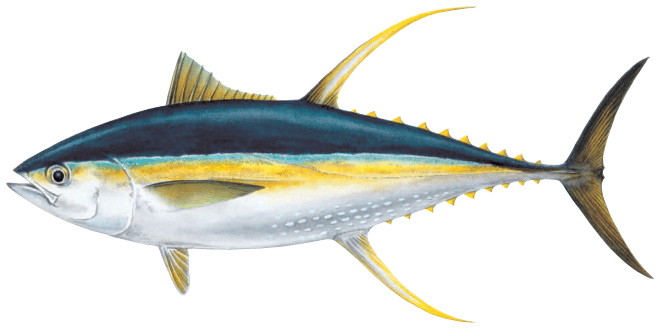
\includegraphics[width=4cm]{fish_yellowfin}
  \end{textblock}
\end{frame}

% ______________________________________________________________________________

\begin{frame}{Overview}
  \begin{itemize}
    \item[] {\bf\darkblue Background} \comment{2020 assessment}\\[5ex]
    \item[] {\bf\darkblue Review Process} \comment{WCPFC review, panel, format,
      objectives}\\[5ex]
    \item[] {\bf\darkblue Model Development} \comment{phases I--III, 2023
      assessment, regional structure}\\[5ex]
  \end{itemize}
\end{frame}

% ______________________________________________________________________________

\begin{frame}\Large
  \centering\darkgreen\bf
  2020 Assessment
\end{frame}

% ______________________________________________________________________________

\begin{frame}{2020 Assessment Data}\fns
  \vspace{1ex}
  Catches\\[1ex]
  \scriptsize purse seine (blue), miscellaneous (yellow), longline (green),
  pole-and-line (red)\\
  \begin{columns}
    \column{0.6\textwidth}
    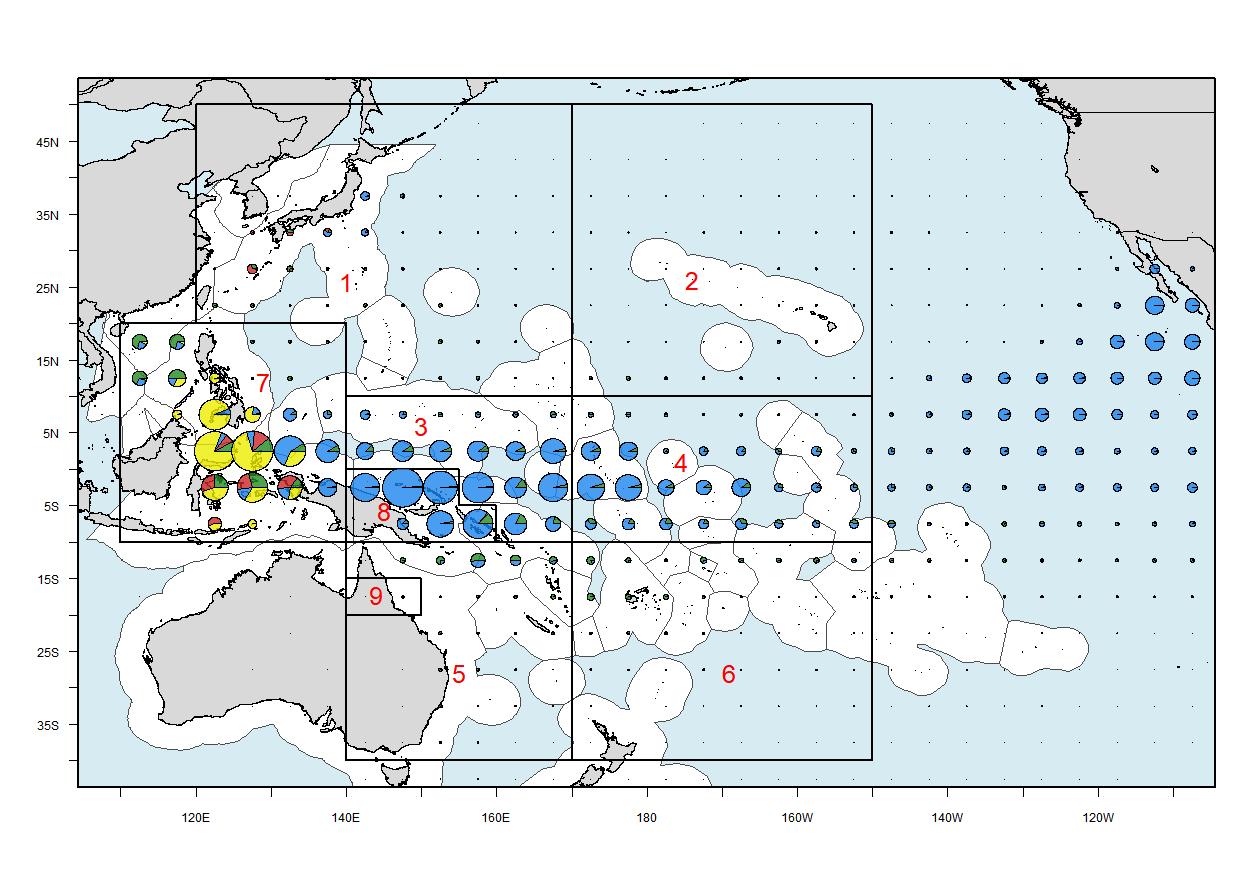
\includegraphics[width=9.5cm]{assmt_fig_05_catch_map}
    \column{0.35\textwidth}~~~
    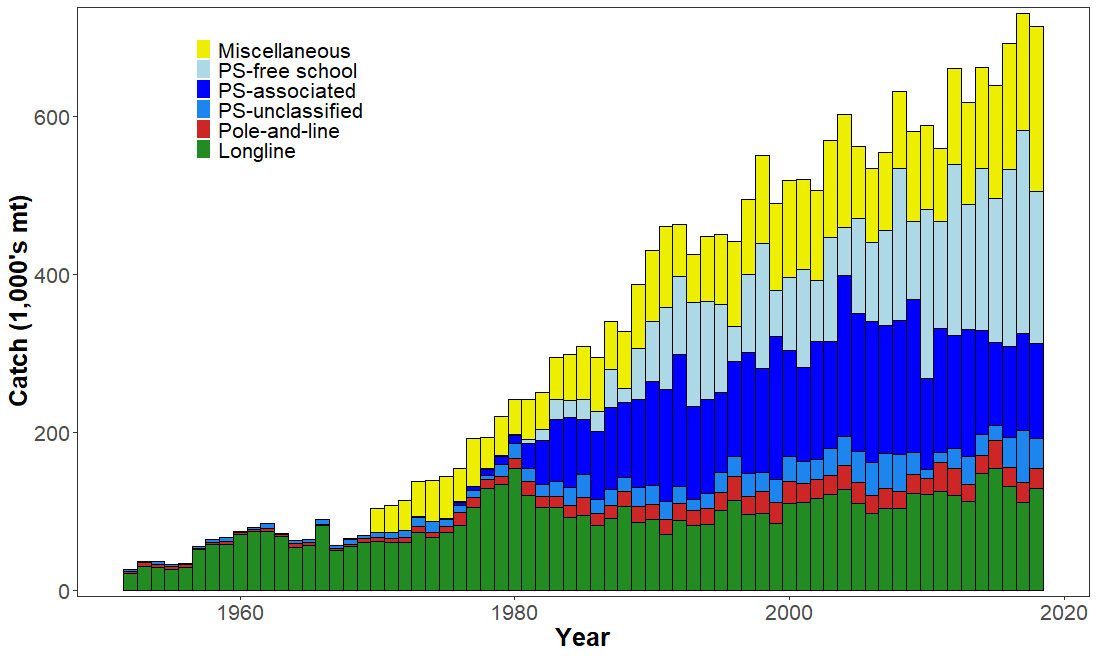
\includegraphics[width=5cm]{assmt_fig_03_catch}
  \end{columns}
\end{frame}

% ______________________________________________________________________________

\begin{frame}{2020 Assessment Data}\fns
  \vspace{1ex}
  Catches\\[3ex]
  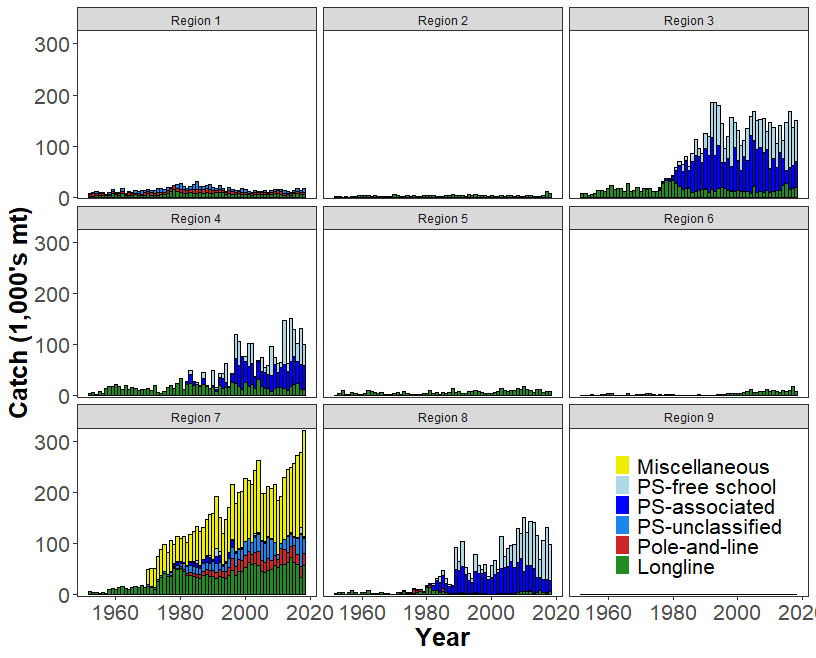
\includegraphics[width=8cm]{assmt_fig_04_catch_region}~~~
  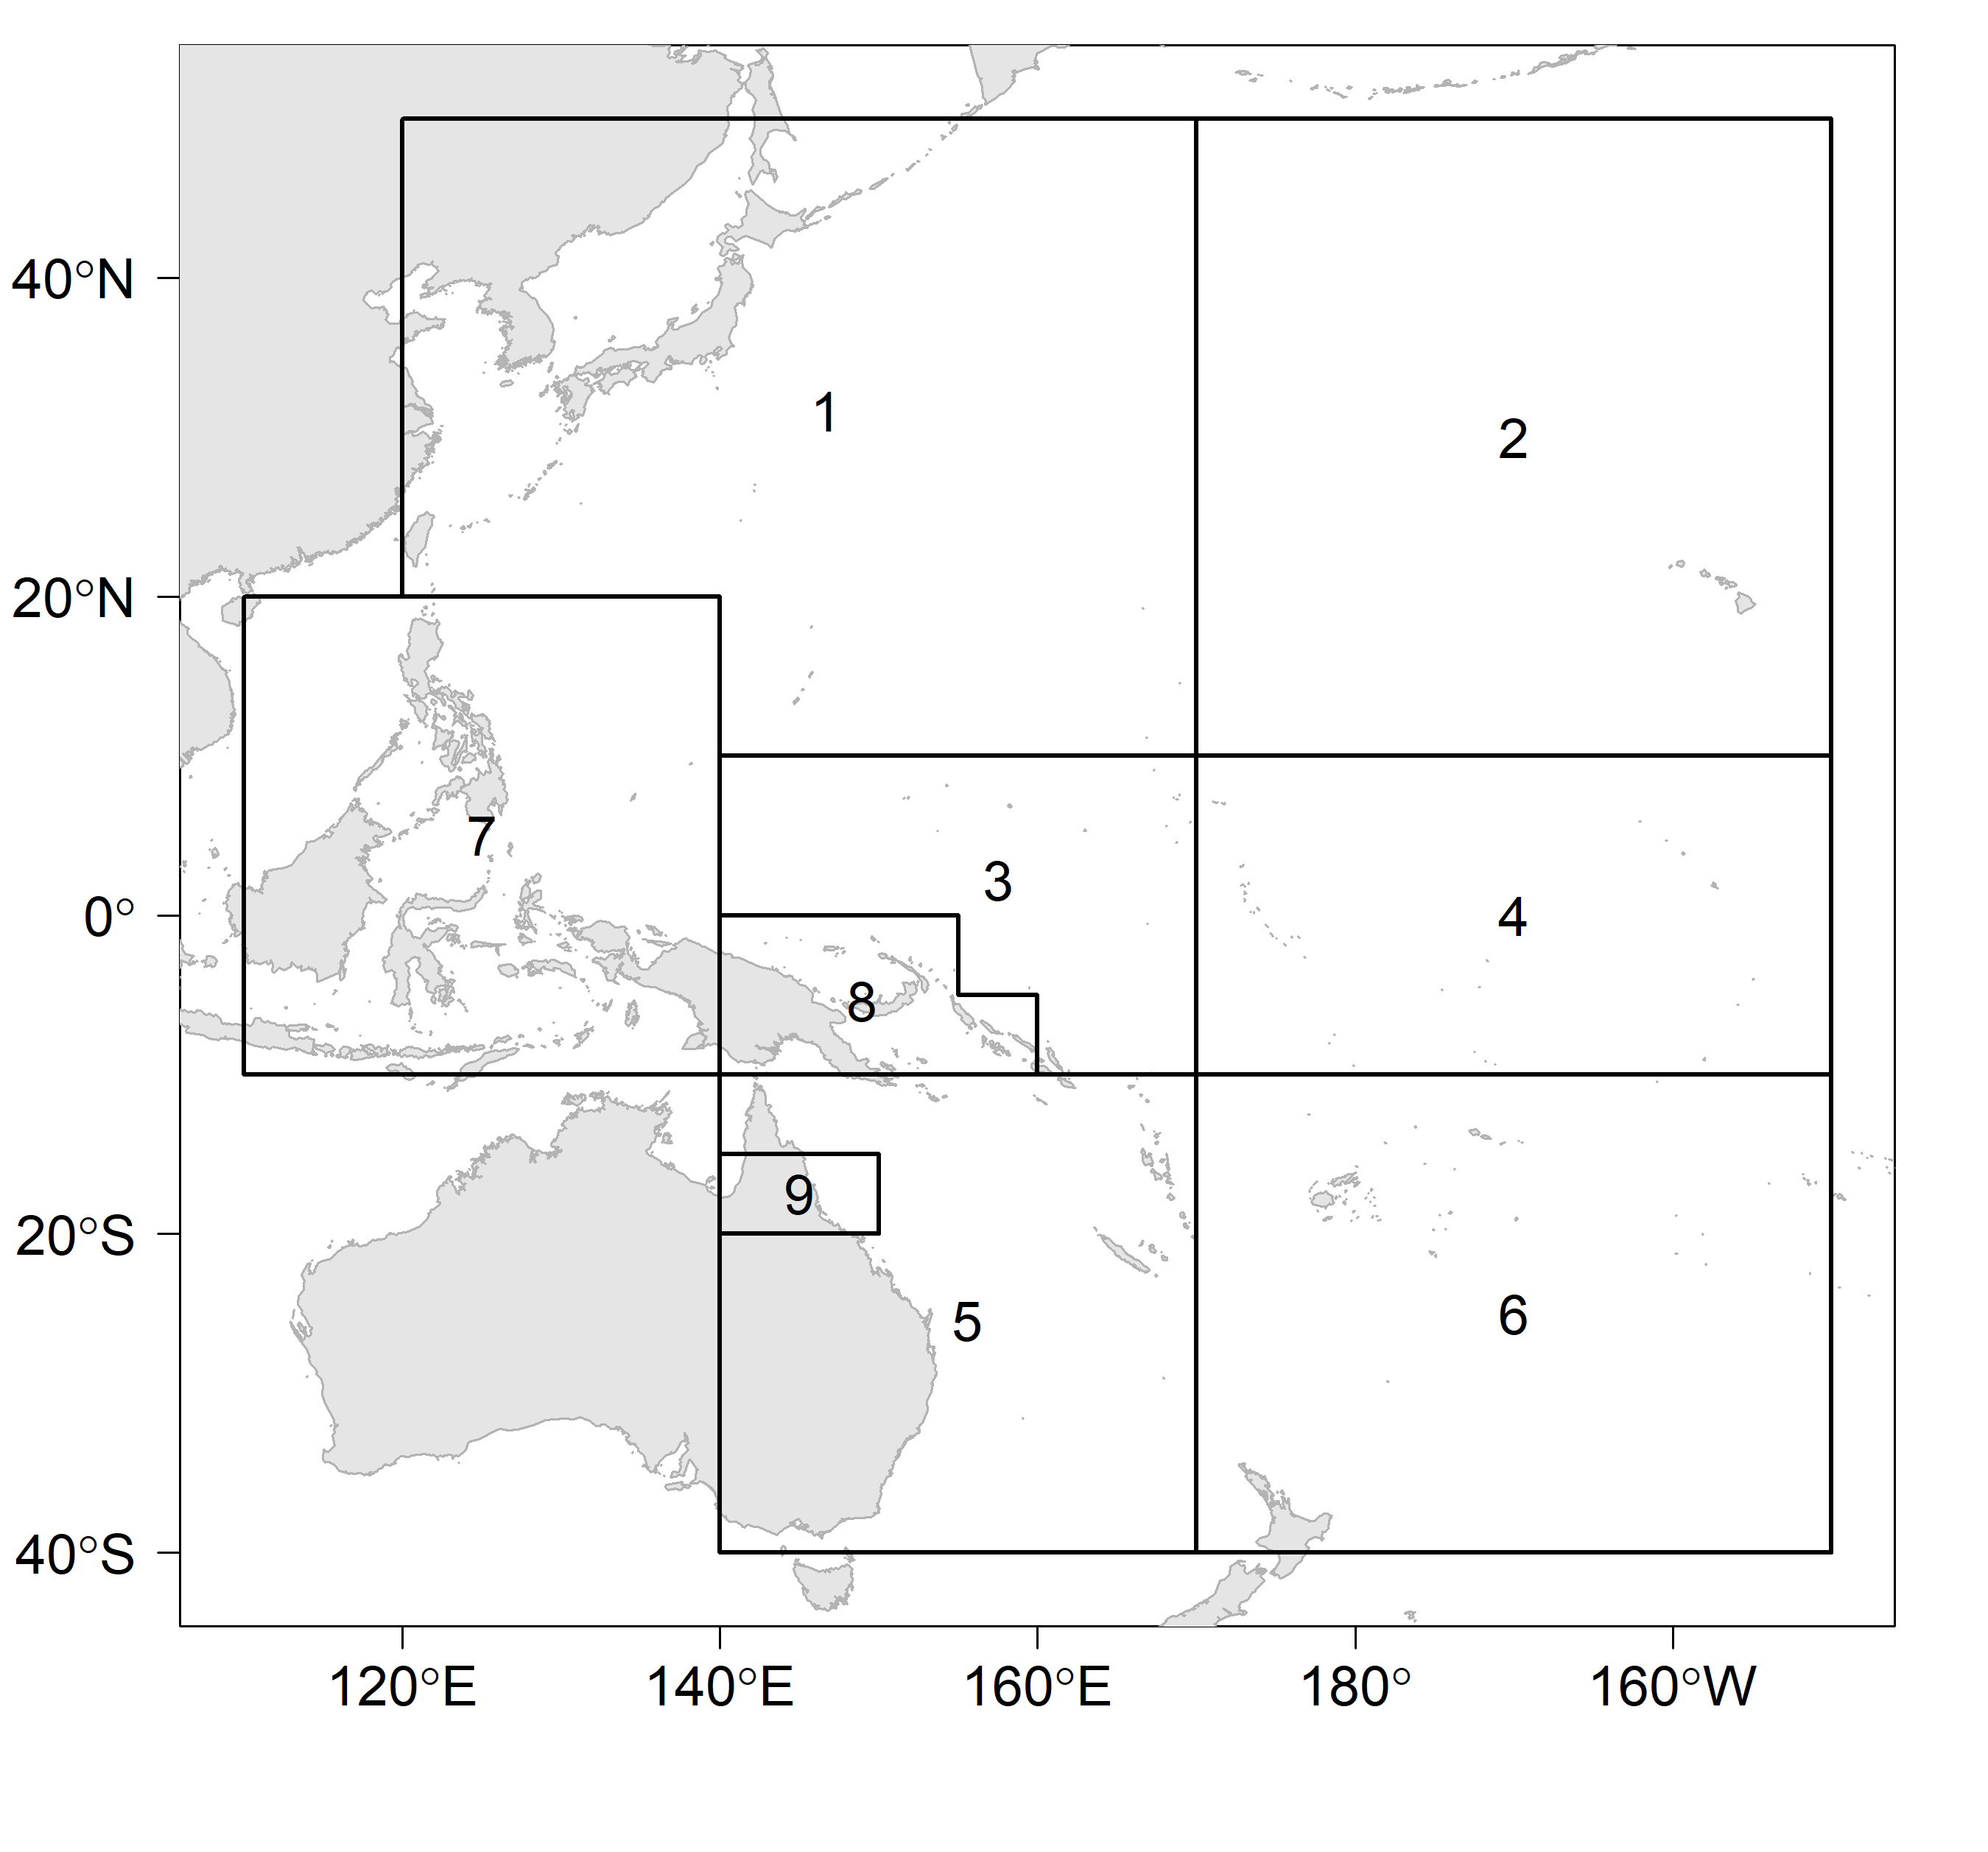
\includegraphics[width=6.5cm]{assmt_fig_01_map}
  \vspace{1ex}
\end{frame}

% ______________________________________________________________________________

\begin{frame}{2020 Assessment Data}\fns
  \vspace{1ex}
  Catches\\[0ex]
  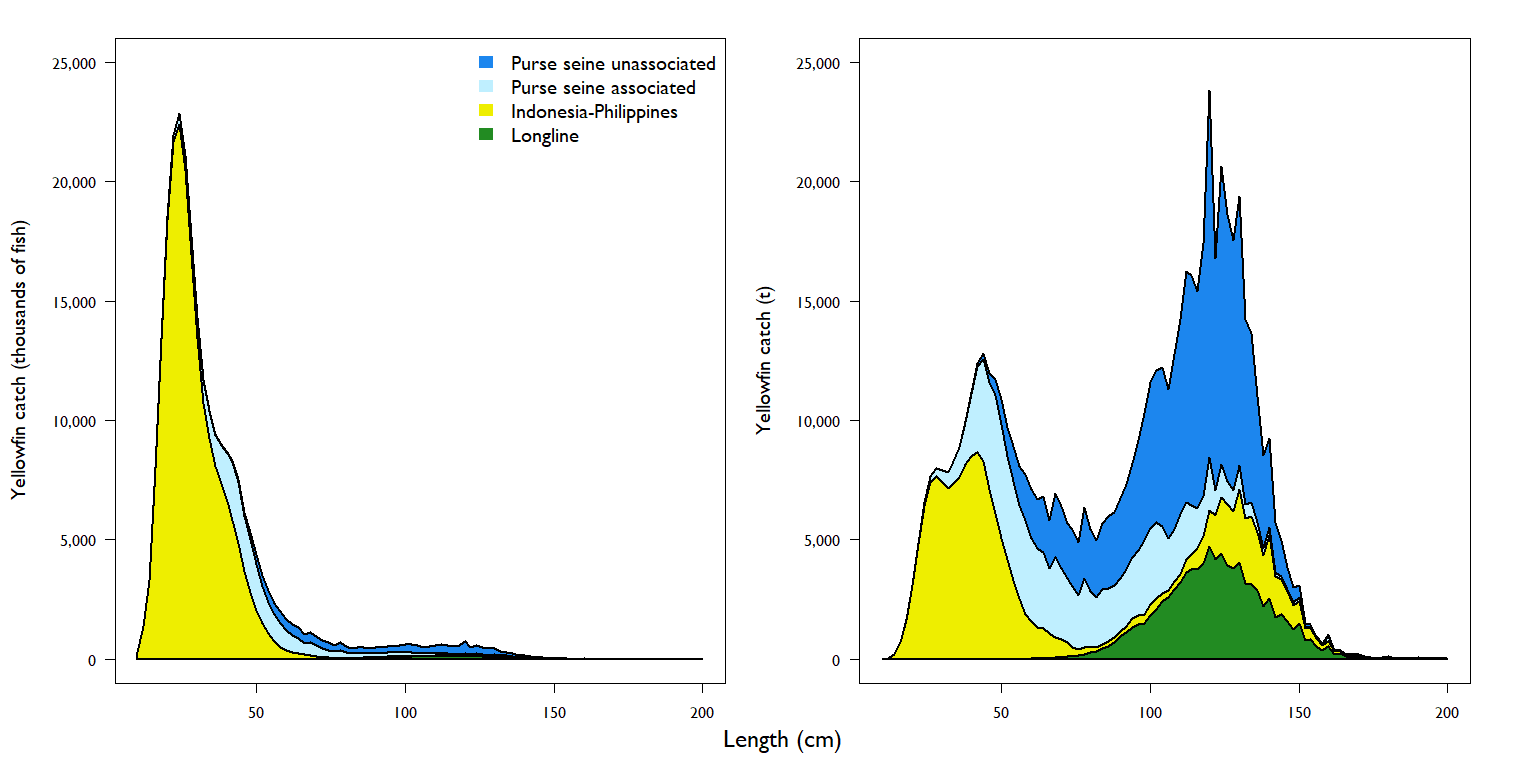
\includegraphics[width=14cm]{tfar_fig_08_catch_length}
  \vspace{1ex}
\end{frame}
% ______________________________________________________________________________

\begin{frame}{2020 Assessment Data}\fns
  \vspace{1ex}
  Tagging Data\\[2ex]
  \begin{columns}
    \column{0.5\textwidth}
    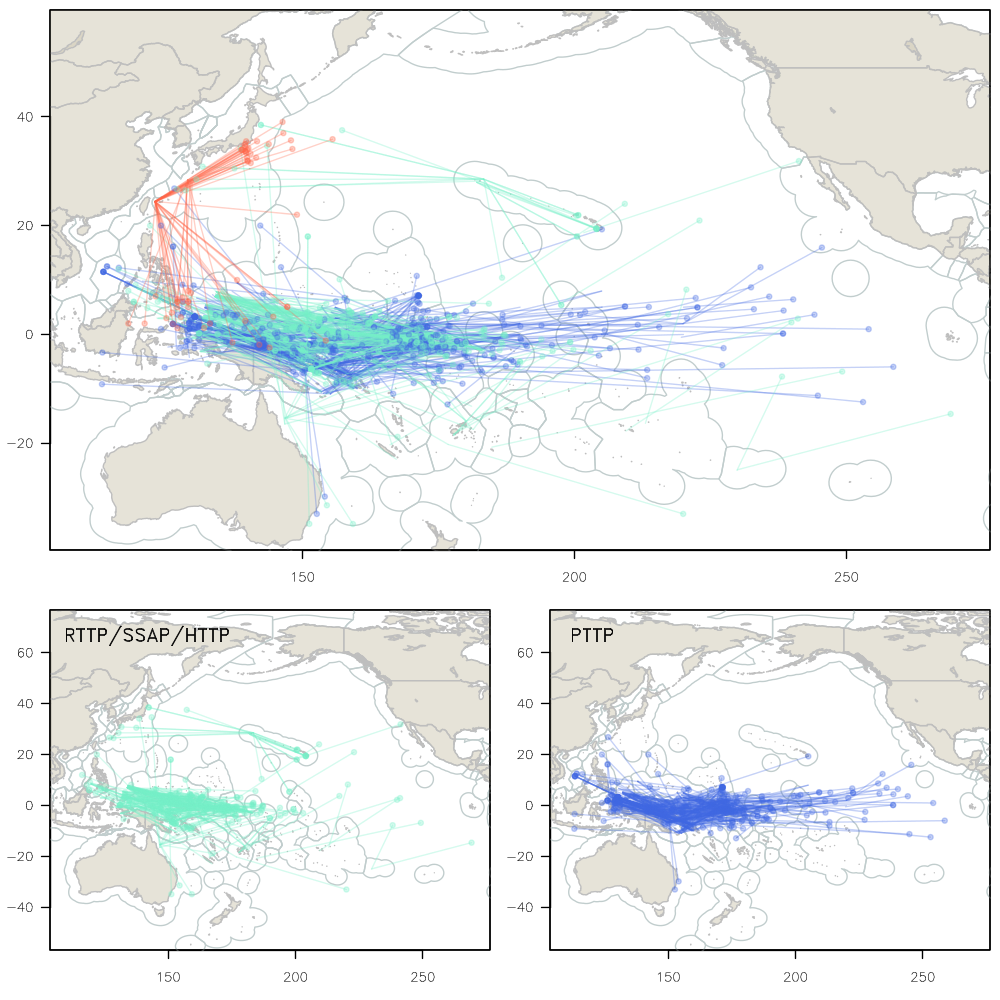
\includegraphics[width=6.5cm]{assmt_fig_02_tag_map}
    \column{0.5\textwidth}\tiny
    \begin{tabular}{llrrr}
      \hline
      Program & Years      & Groups & Releases & Recoveries\I{2.4ex}\\[0.4ex]
      \hline
      JPTP    & 1999--2017 &     58 &    10551 &       1024\I{2.6ex}\\[0.6ex]
      PTTP    & 2006--2017 &     53 &    79339 &      17002\\[0.6ex]
      RTTP    & 1989--1995 &     34 &    26235 &       4380\\
      \hline
    \end{tabular}
  \end{columns}
  \vspace{2ex}
\end{frame}

% ______________________________________________________________________________

\begin{frame}{2020 Assessment Data}\fns
  \vspace{1ex}
  CPUE\\
  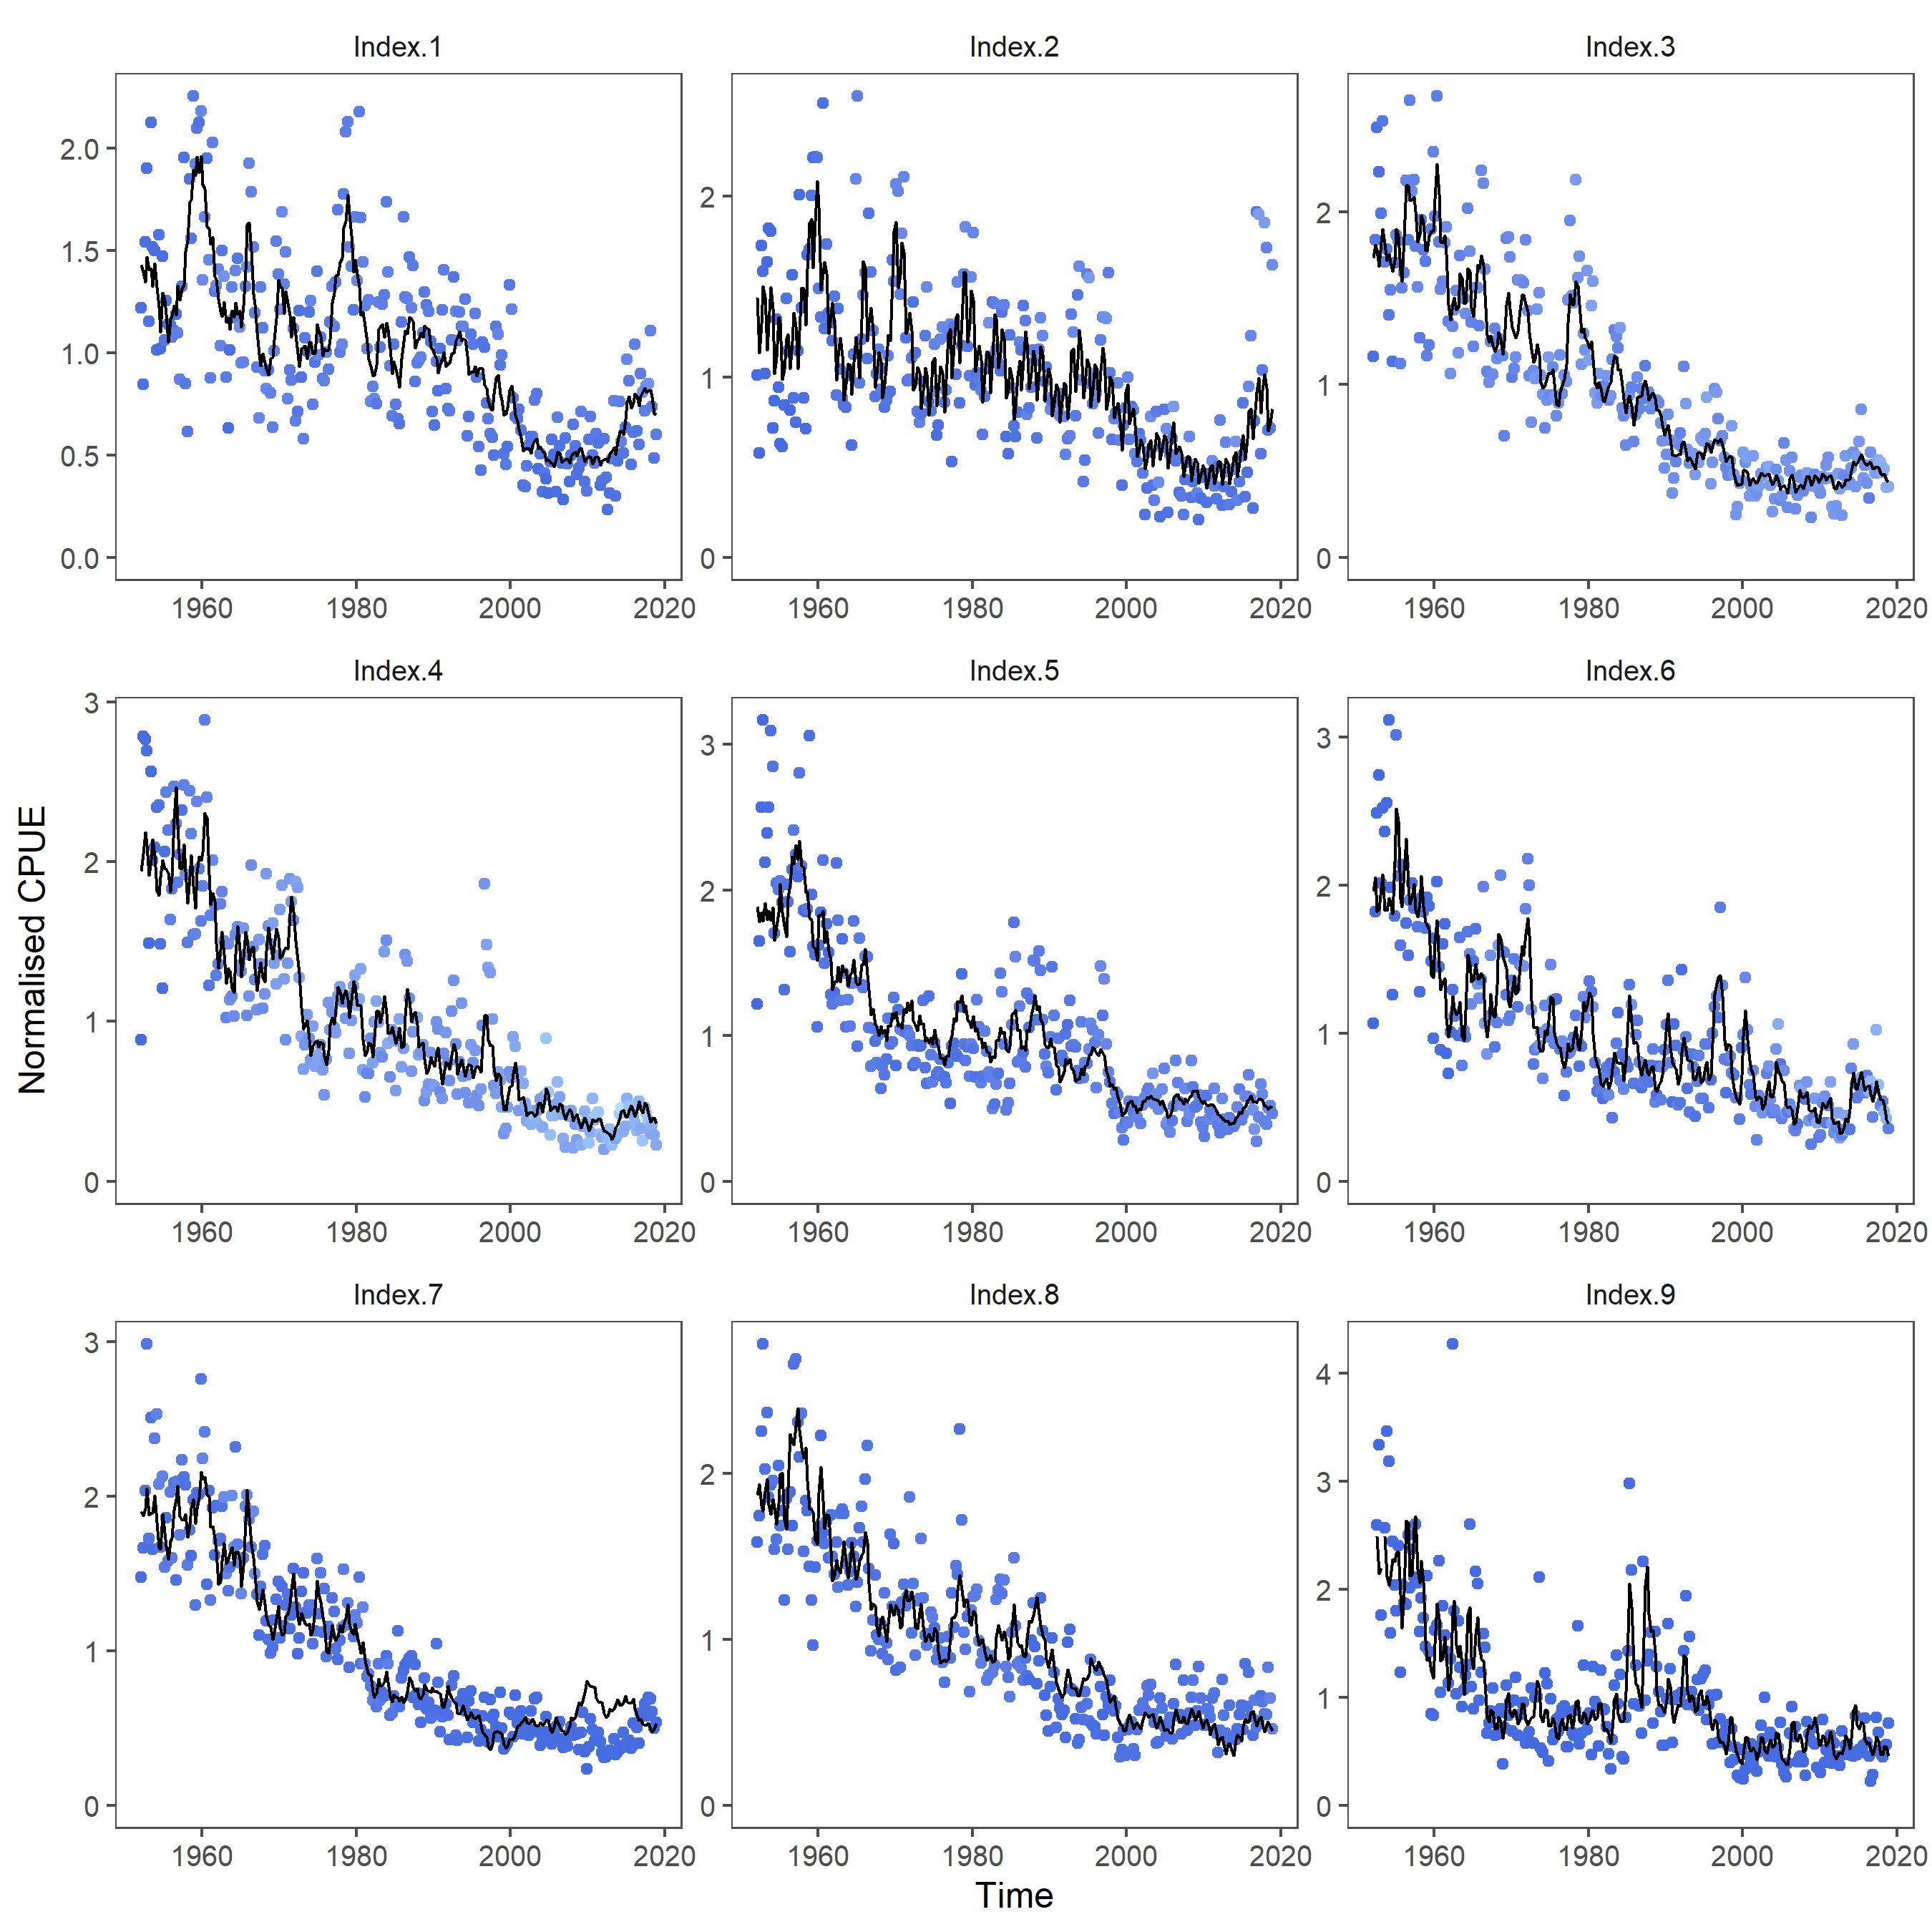
\includegraphics[width=7cm]{fig_16_cpue}
\end{frame}
% ______________________________________________________________________________

\begin{frame}{2020 Assessment Data}\fns
  \vspace{1ex}
  CPUE\\[1ex]
  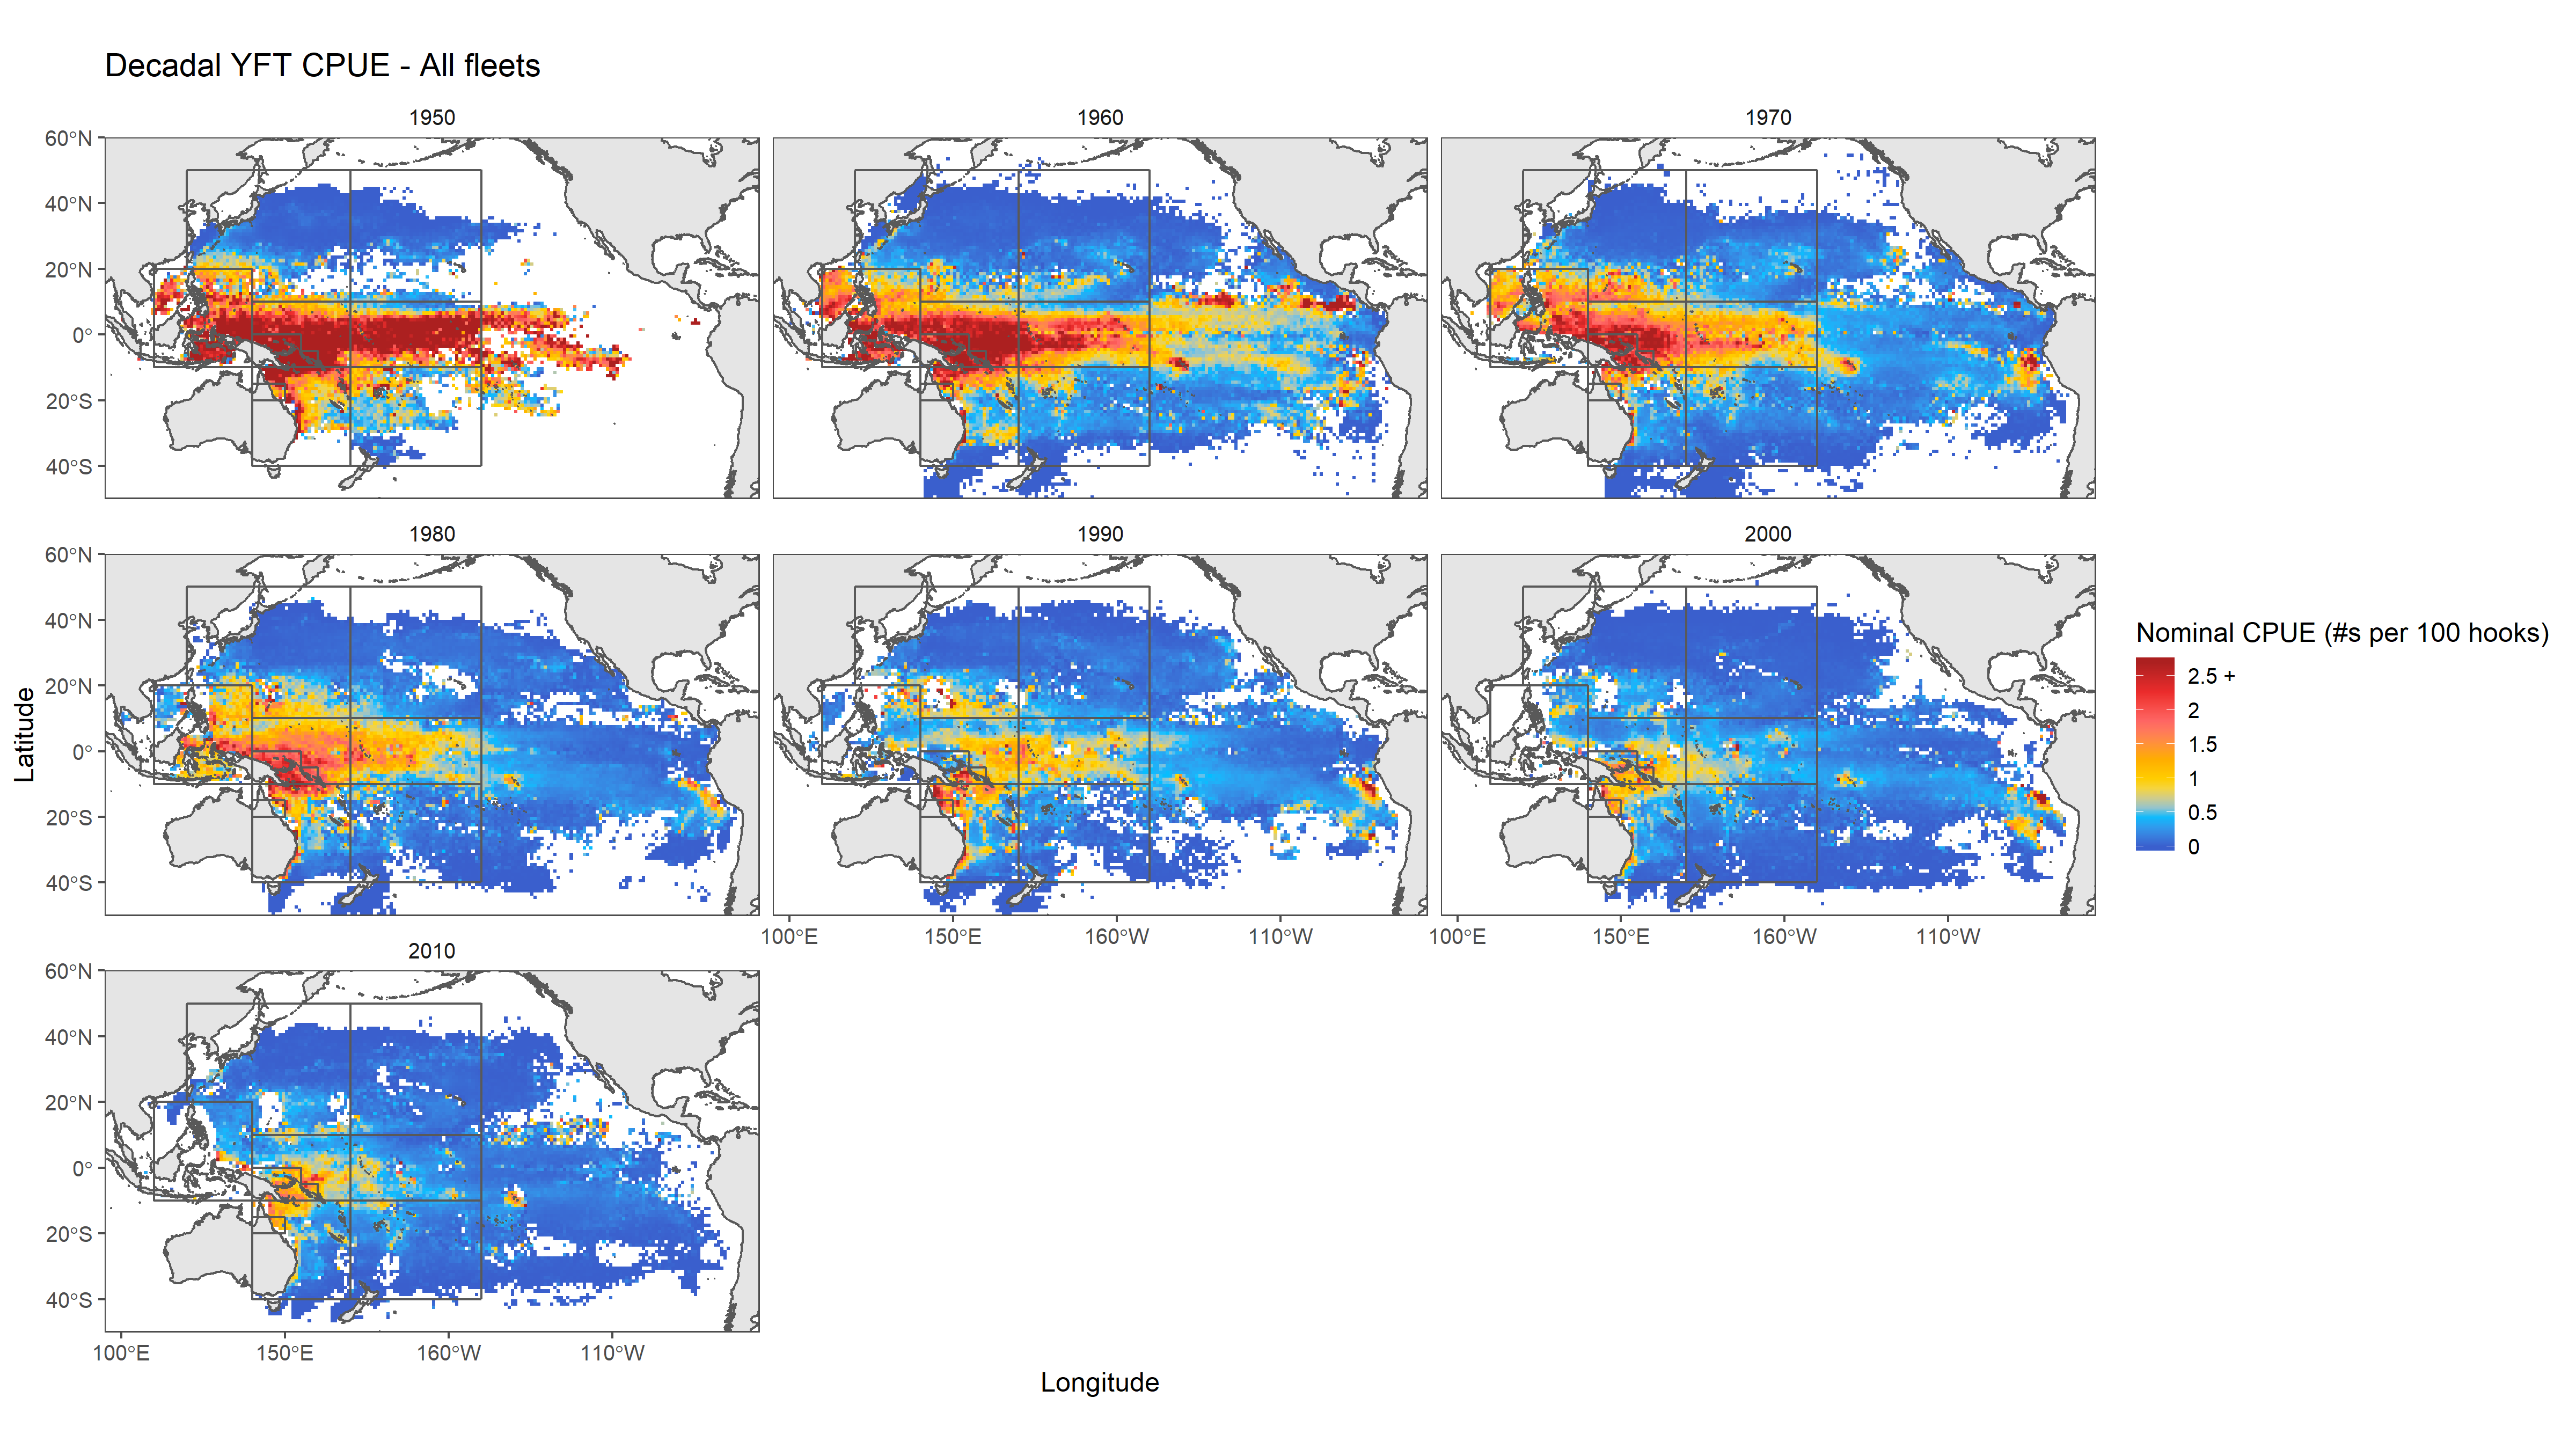
\includegraphics[width=12cm]{fig_08_cpue_map}
  \vspace{1ex}
\end{frame}
% ______________________________________________________________________________

\begin{frame}{2020 Assessment Model}\small
  Multifan-CL with\\[1ex]
  \begin{itemize}
    \item[] 9 regions\\[2ex]
    \item[] 1962--2018, quarterly time step\\[2ex]
    \item[] 32 extraction fisheries\\[2ex]
    \item[] 9 index fisheries, VAST analysis of longline CPUE\\[2ex]
    \item[] 11671 estimated parameters\\[2ex]
    \item[] 72 models in uncertainty grid (steepness, growth, sample size, tag
    mixing)\\[2ex]
  \end{itemize}
\end{frame}

% ______________________________________________________________________________

\begin{frame}{2020 Assessment Results}\fns
  \vspace{1ex}
  Spawning Potential and Recruitment\\[4ex]
  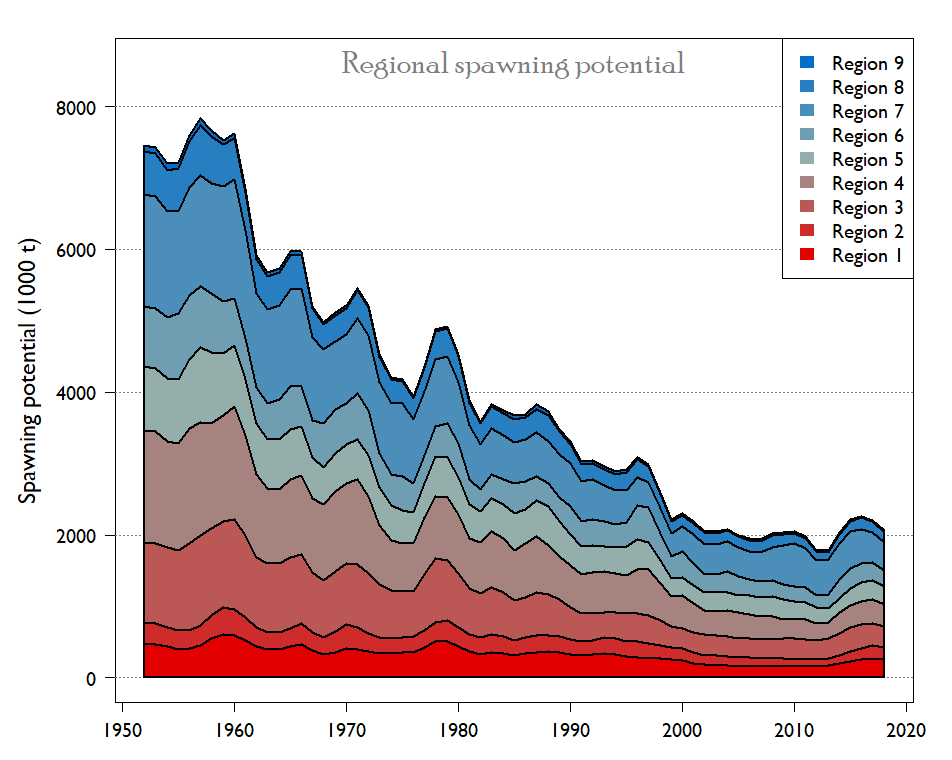
\includegraphics[width=7cm]{tfar_fig_09a_ssb}~~~~~
  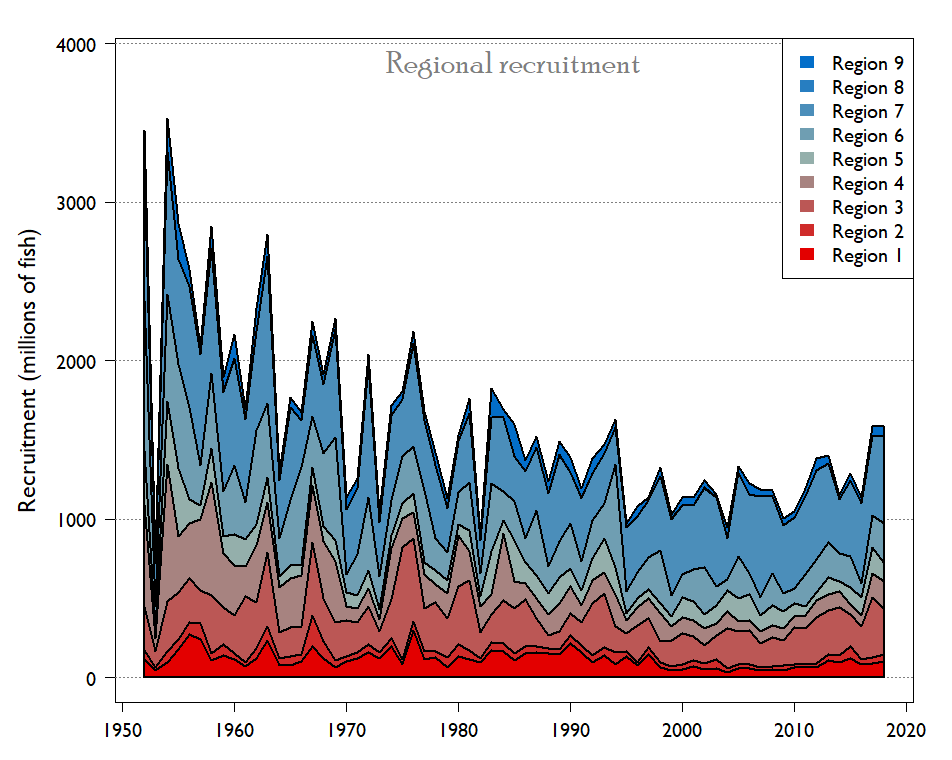
\includegraphics[width=7cm]{tfar_fig_09b_recruitment}
  \vspace{3ex}
\end{frame}

% ______________________________________________________________________________

\begin{frame}{2020 Assessment Results}\fns
  \vspace{1.5ex}
  Fishing Mortality and Stock Status\\[1ex]
  \begin{columns}
    \column{0.5\textwidth}
    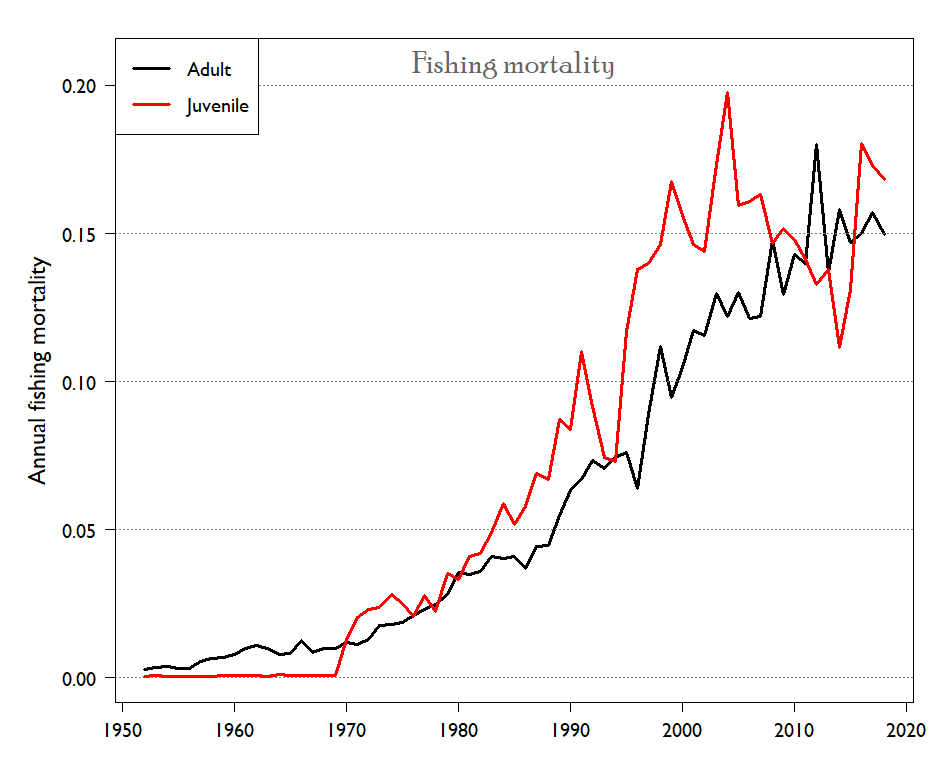
\includegraphics[width=8cm]{tfar_fig_09c_fmortality}~~~
    \column{0.5\textwidth}
    \centering
    \h{8ex}$n=72$ models\I{3ex}\\[1ex]
    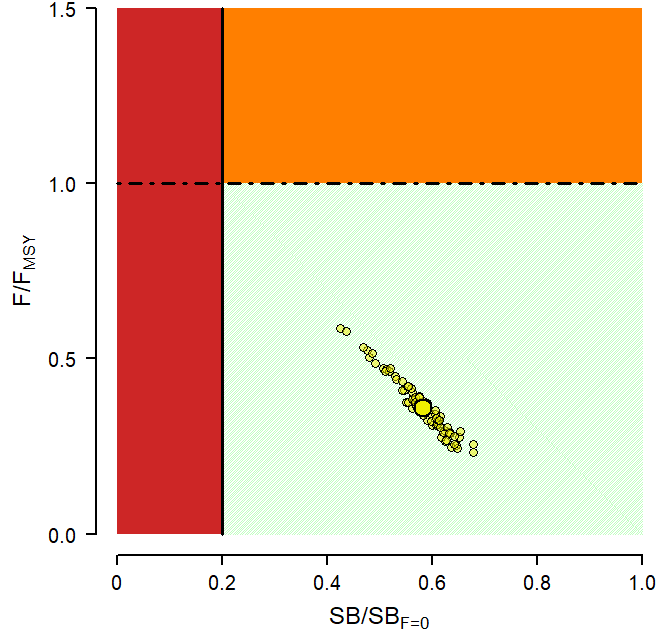
\includegraphics[width=6.5cm]{tfar_fig_09d_majuro_crop}
  \end{columns}
  \vspace{2ex}
\end{frame}

% ______________________________________________________________________________

\begin{frame}{2020 Assessment Results}\fns
  \vspace{1ex}
  Stock Status, Differences Between Assessments\\[4ex]
  \begin{columns}
    \column{0.45\textwidth}
    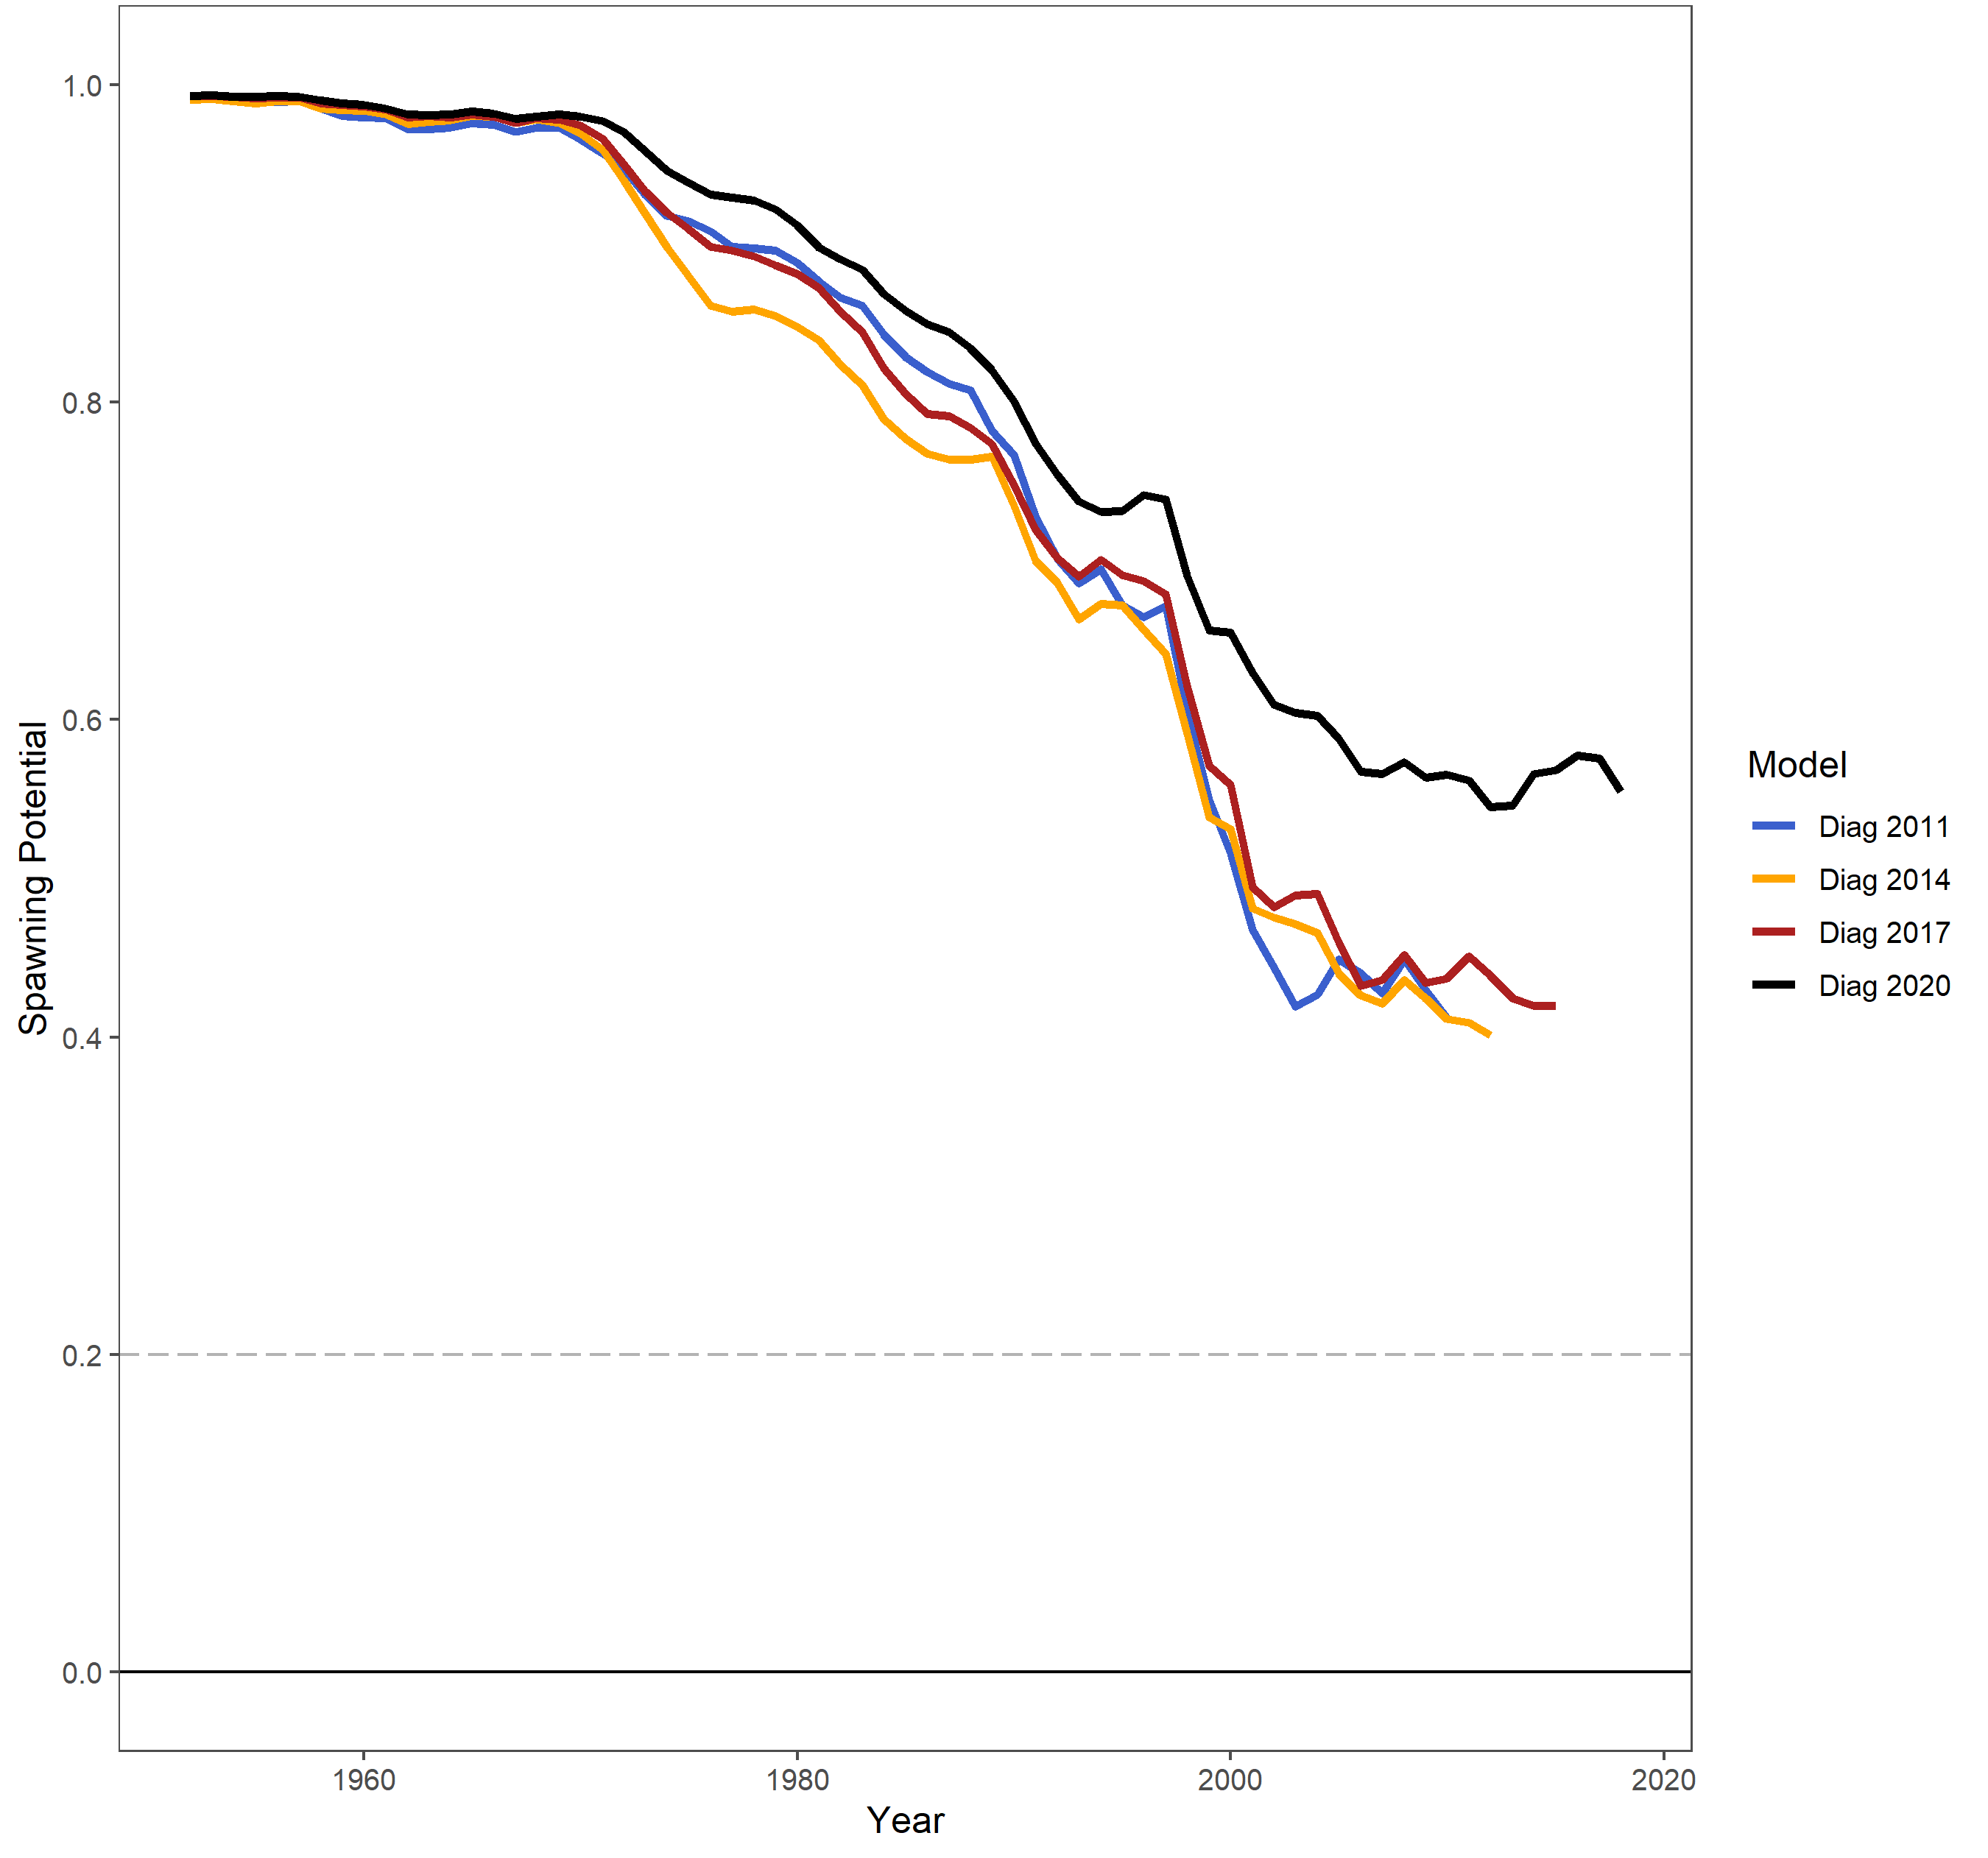
\includegraphics[width=6.5cm]{assmt_fig_a4_historical_crop}
    \column{0.55\textwidth}
    ~~~~Considerably more optimistic than\\
    ~~~~previous assessments --- why?\\[5ex]
    ~~~~New features in the 2020 assessment\\[1ex]
    \begin{itemize}\scriptsize
      \item[-] Growth data from both otoliths and tag recaptures
      \item[-] Richards growth model
      \item[-] Updated spawning potential based on maturity at length
      \item[-] `Index fishery' approach with 9 VAST CPUE series
      \item[-] `Pseudo catch conditioned' estimation of F
      \item[-] Increased maximum age from 7 to 10 years old
      \item[-] Uncoupled selectivity parameters between regions
    \end{itemize}
    \vspace{6ex}
  \end{columns}
  \vspace{1.5ex}
\end{frame}

% ______________________________________________________________________________

\begin{frame}{2020 Assessment Results}\fns
  Stepwise and Retrospectives\\[3ex]
  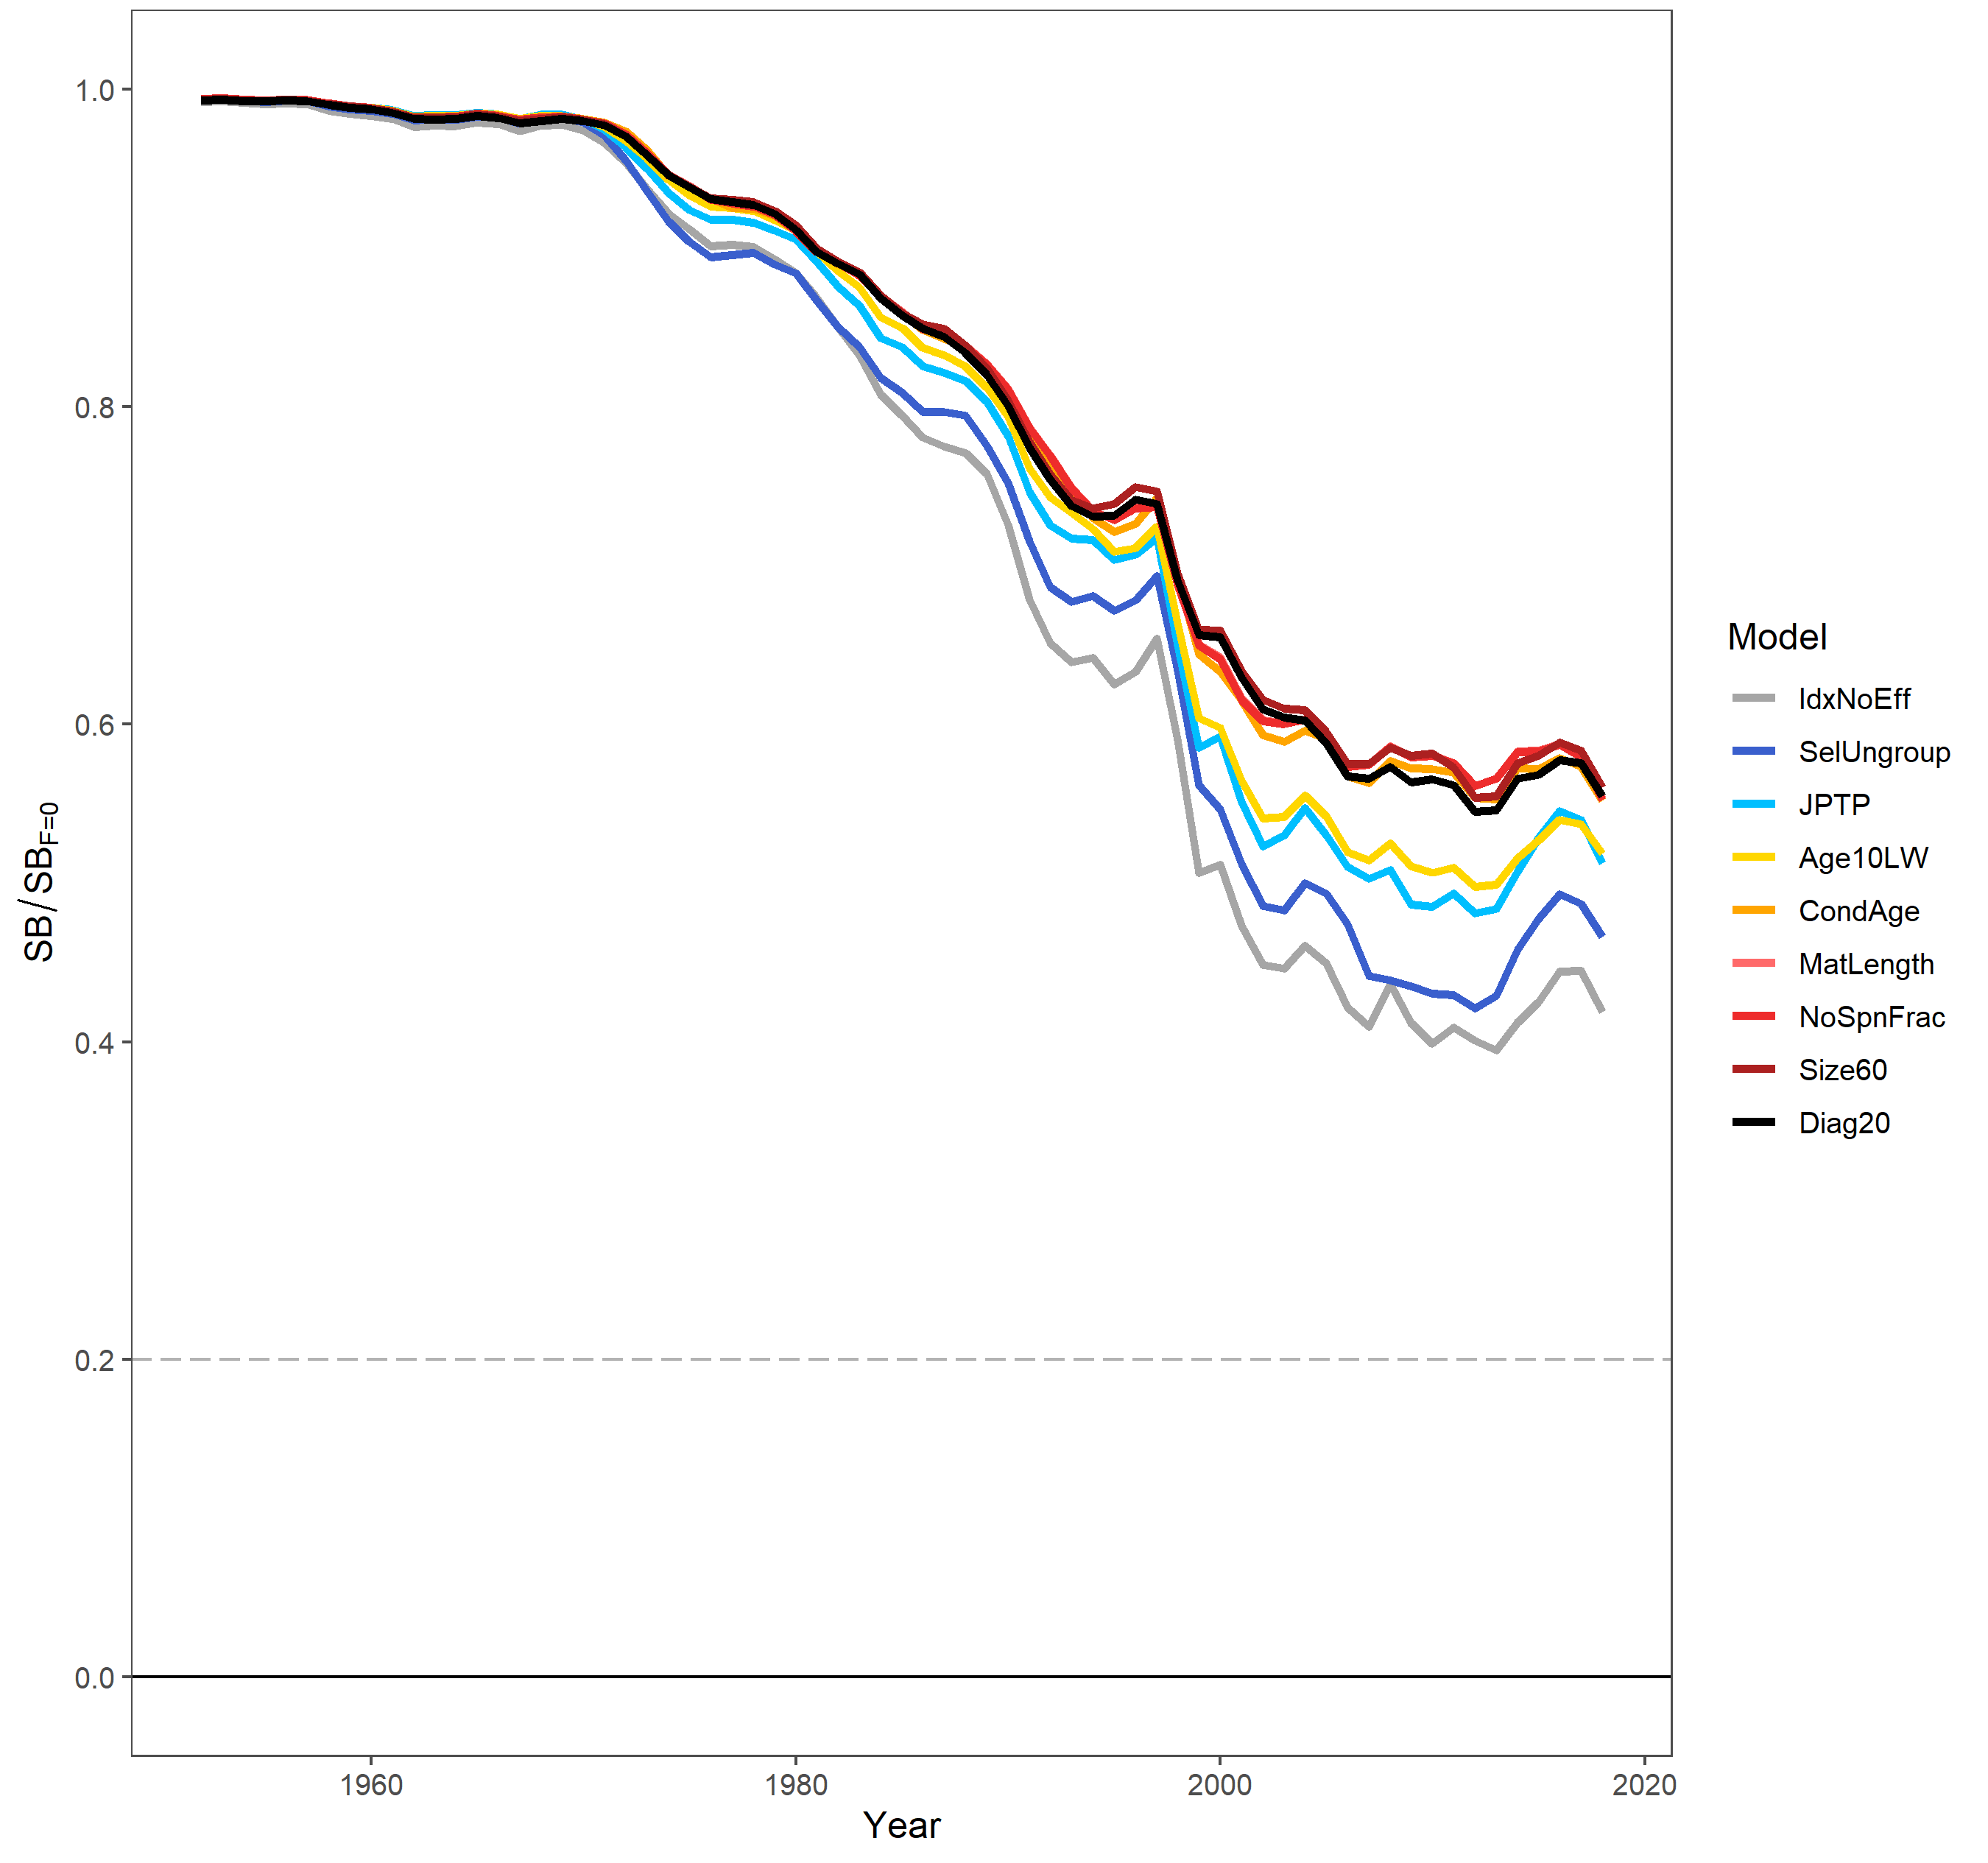
\includegraphics[width=6.8cm]{fig_14b_stepwise_crop}~~~~~
  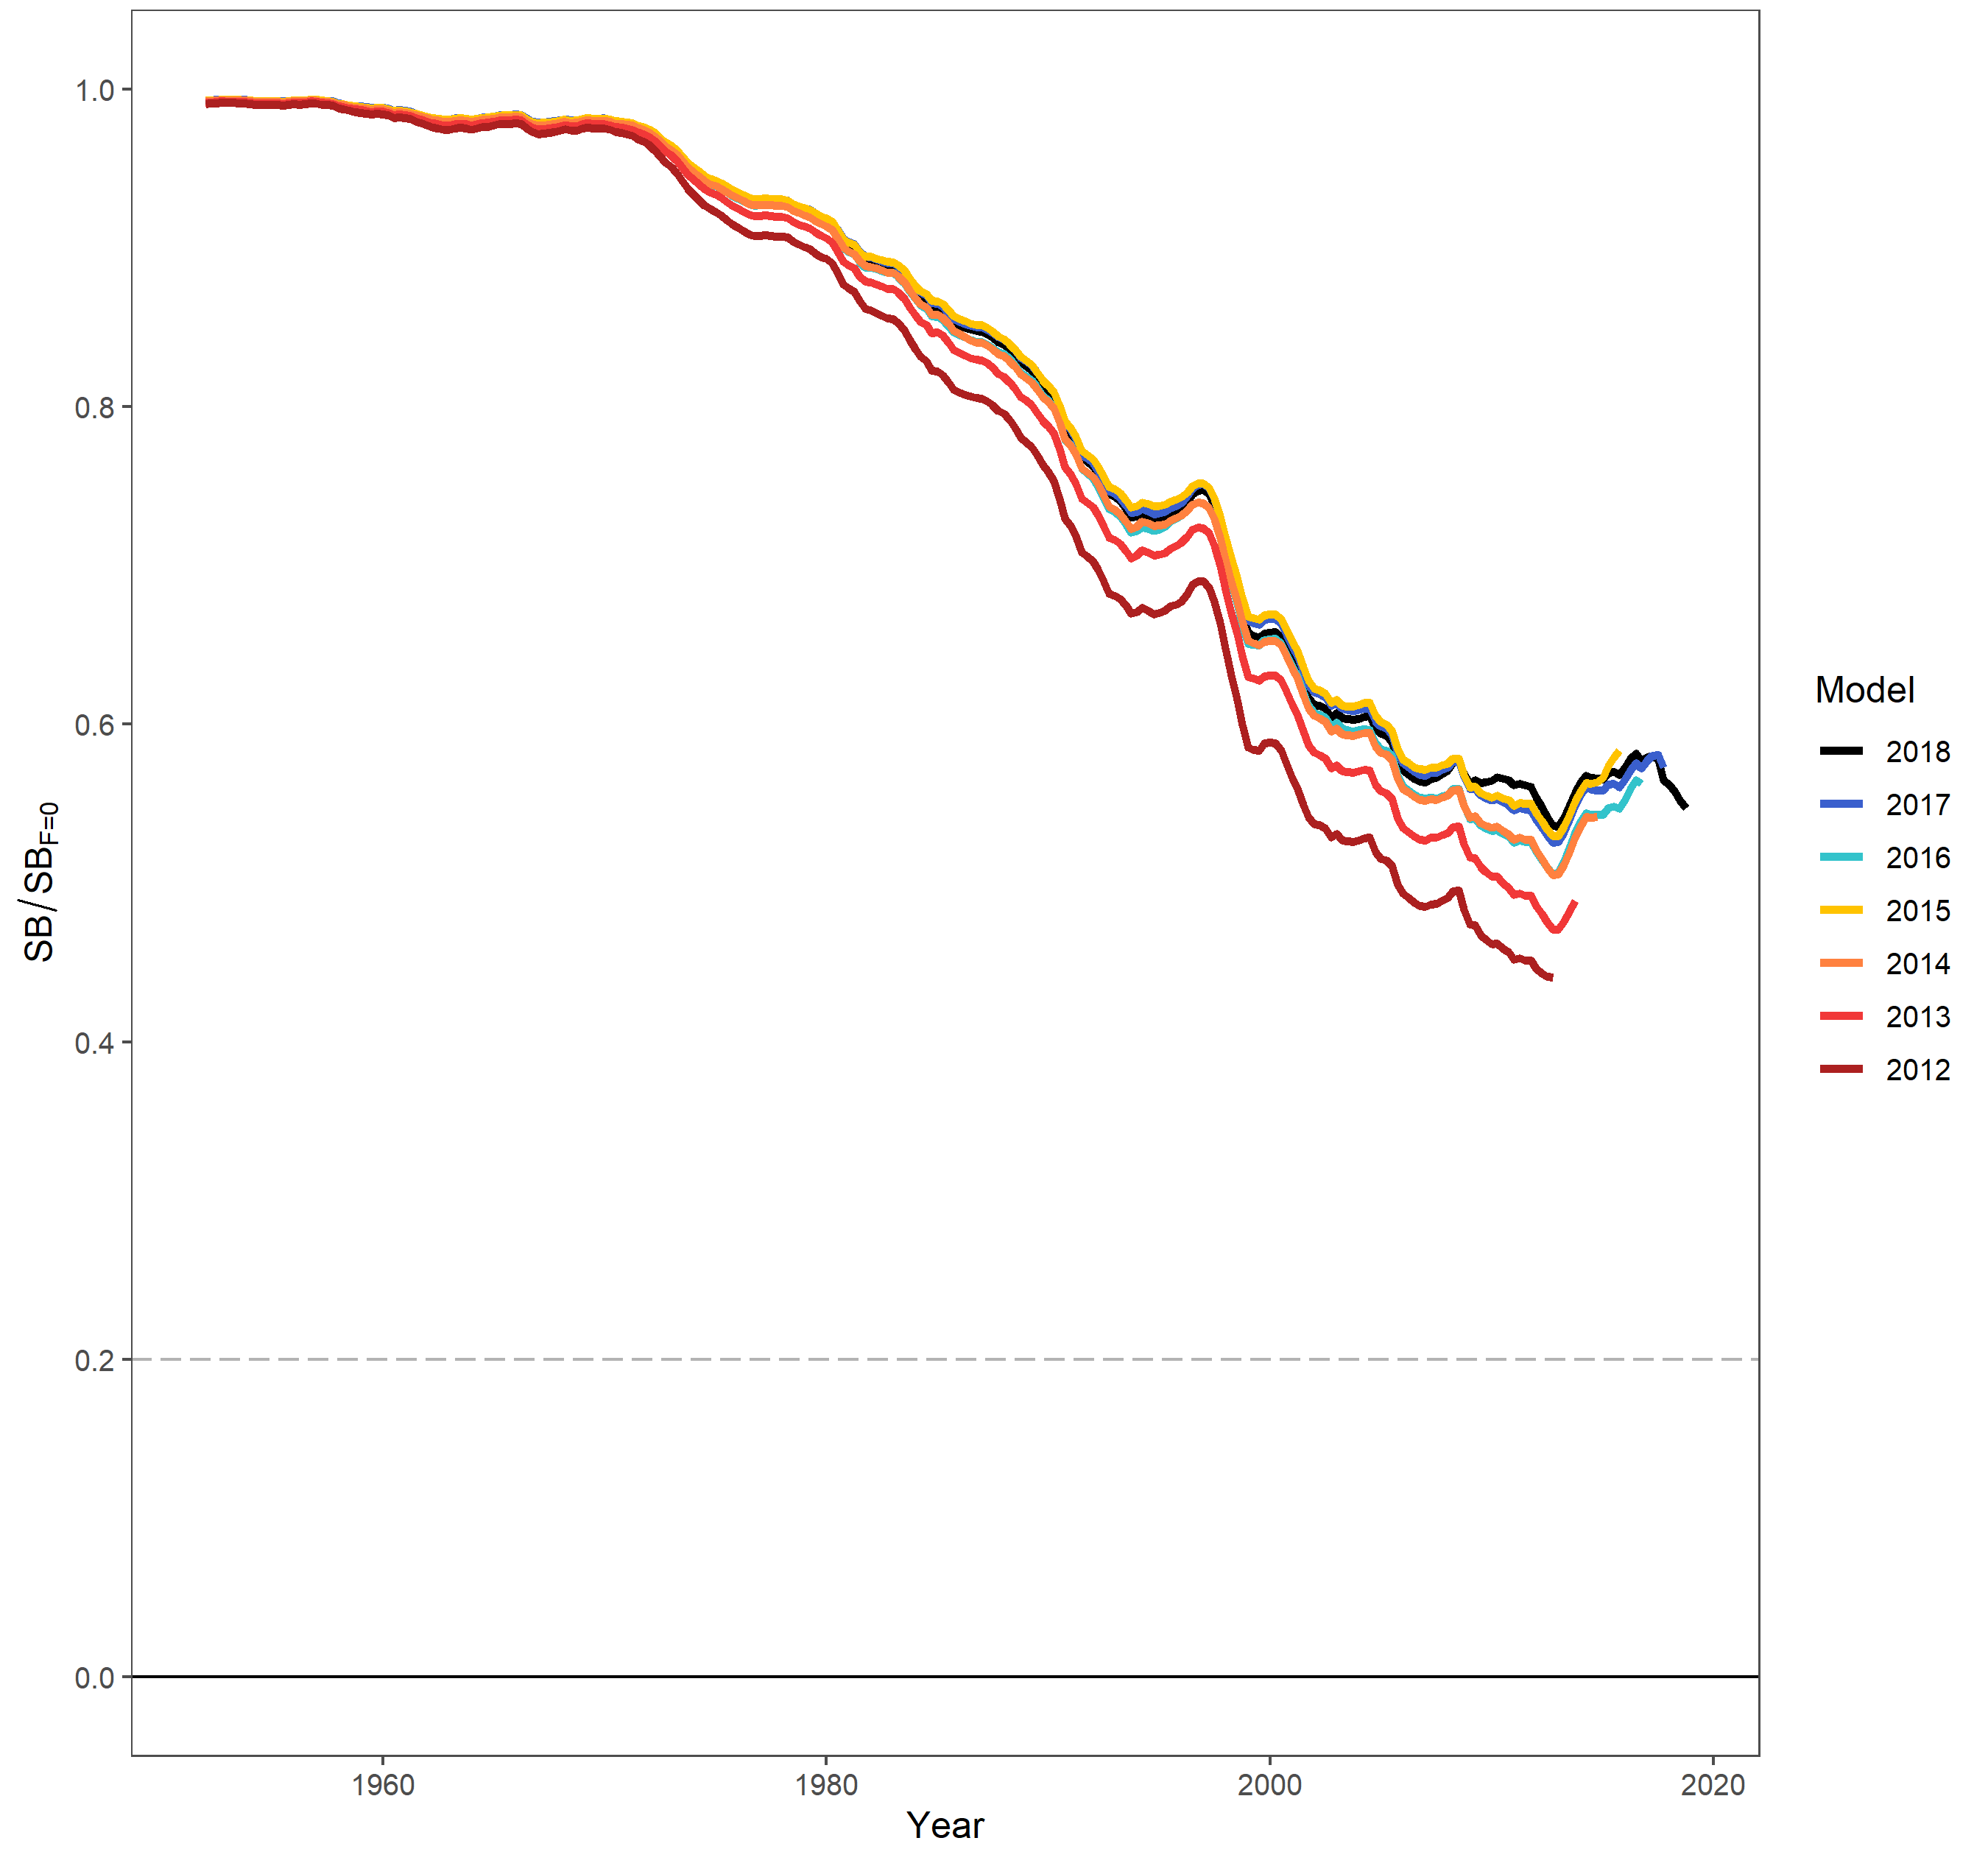
\includegraphics[width=6.8cm]{fig_a3b_retro_crop}
\end{frame}

% ______________________________________________________________________________

\begin{frame}\Large
  \centering\darkgreen\bf
  Review Process
\end{frame}

% ______________________________________________________________________________

\begin{frame}{Review Process and Panel}\small
  WCPFC review requested by SC16 to examine possible improvements\\[0.2ex]
  for the 2023 assessment, SC17 approved Terms of Reference\\[4ex]
  Review panel: Mark Maunder, Jim Ianelli, André Punt (chair)\\[5ex]
  \begin{columns}
    \column{0.2\textwidth}\centering
    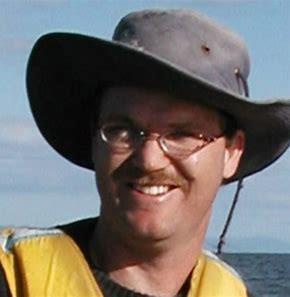
\includegraphics[height=2.5cm]{panel_mark}
    \column{0.2\textwidth}\centering
    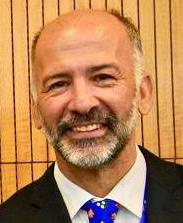
\includegraphics[height=2.5cm]{panel_jim}
    \column{0.2\textwidth}\centering
    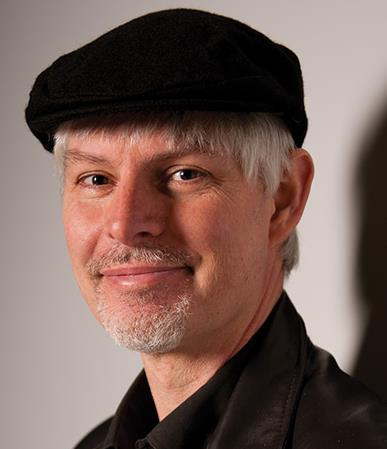
\includegraphics[height=2.5cm]{panel_andre}
  \end{columns}
  \vspace{6ex}
\end{frame}

% ______________________________________________________________________________

\begin{frame}{Review Panel}\fns
  \vspace{2ex}
  \begin{columns}
    \column{0.2\textwidth}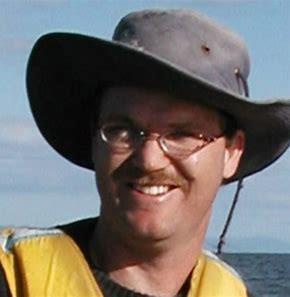
\includegraphics[height=2.5cm]{panel_mark}
    \column{0.2\textwidth}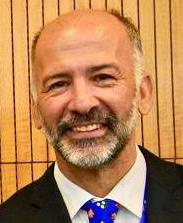
\includegraphics[height=2.5cm]{panel_jim}
    \column{0.2\textwidth}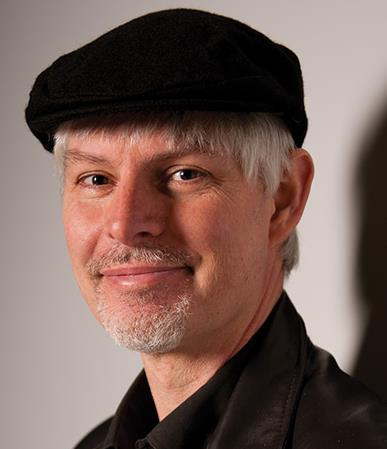
\includegraphics[height=2.5cm]{panel_andre}
  \end{columns}
  \vspace{3ex}
  \h{7ex}{\darkgreen An artist, an economist, and a biologist entered a stock
    assessment review meeting...}\\[2ex]
  \h{7ex}The Biologist [squeezes a fish and some eggs come out]:\\[-1ex]
  \begin{quote}\h{4ex}
    ``There are still some spawners left, so the stock should be fine''\\[3ex]
  \end{quote}
  \h{7ex}The Economist [looks at the financial report]:\\[-1ex]
  \begin{quote}\h{4ex}
    ``They are still making some money, so the stock should be fine''\\[3ex]
  \end{quote}
  \h{7ex}The Artist [looks at the stock assessment report]:\\[-1ex]
  \begin{quote}\h{4ex}
    ``These are quite good, but I have seen better abstract paintings''\\[3ex]
  \end{quote}
\end{frame}

% ______________________________________________________________________________

\begin{frame}{Review Format}\small
  Continuous format: quick chats (milestones) in December 2021, April 2022, June
  2022\\[5ex]
  Main review meeting in Noumea 7--13 September 2022\\[5ex]
  Review panel reports back to SC\\[5ex]
  Many of the concerns raised for the yellowfin tuna assessment are relevant to
  the bigeye tuna assessment, so the peer review will also have relevance to the
  bigeye assessment\\[5ex]
\end{frame}

% ______________________________________________________________________________

\begin{frame}\Large
  \centering\darkgreen\bf
  Model Development
\end{frame}

% ______________________________________________________________________________

\begin{frame}{Model Development}\fns
  {\darkgreen Phase I} focuses on the use of new features in MFCL:
  \begin{itemize}
    \item Catch-conditioned estimation of F\\[-1ex]
    \item Orthogonal polynomial recruitment\\[-1ex]
    \item Dirichlet-multinomial estimation of sample sizes\\[-1ex]
  \end{itemize}
  \vspace{3ex}
  {\darkgreen Phase II} will focus on regional structure:
  \begin{itemize}
    \item 1 region\\[-1ex]
    \item 4 regions\\[-1ex]
    \item 9 regions\\[-1ex]
  \end{itemize}
  \vspace{3ex}
  {\darkgreen Phase III} will focus on additional issues raised by the review
  panel\\
  and move towards the 2023 assessment\\
  \vspace{3ex}
  The review process and model development can be followed on GitHub:\\
  \qquad\href{https://github.com/PacificCommunity/ofp-sam-yft-review}%
  {\blue PacificCommunity/ofp-sam-yft-review}
  \vspace{3ex}
\end{frame}

% ______________________________________________________________________________

\begin{frame}{Regional Structure}
  \vspace{1ex}
  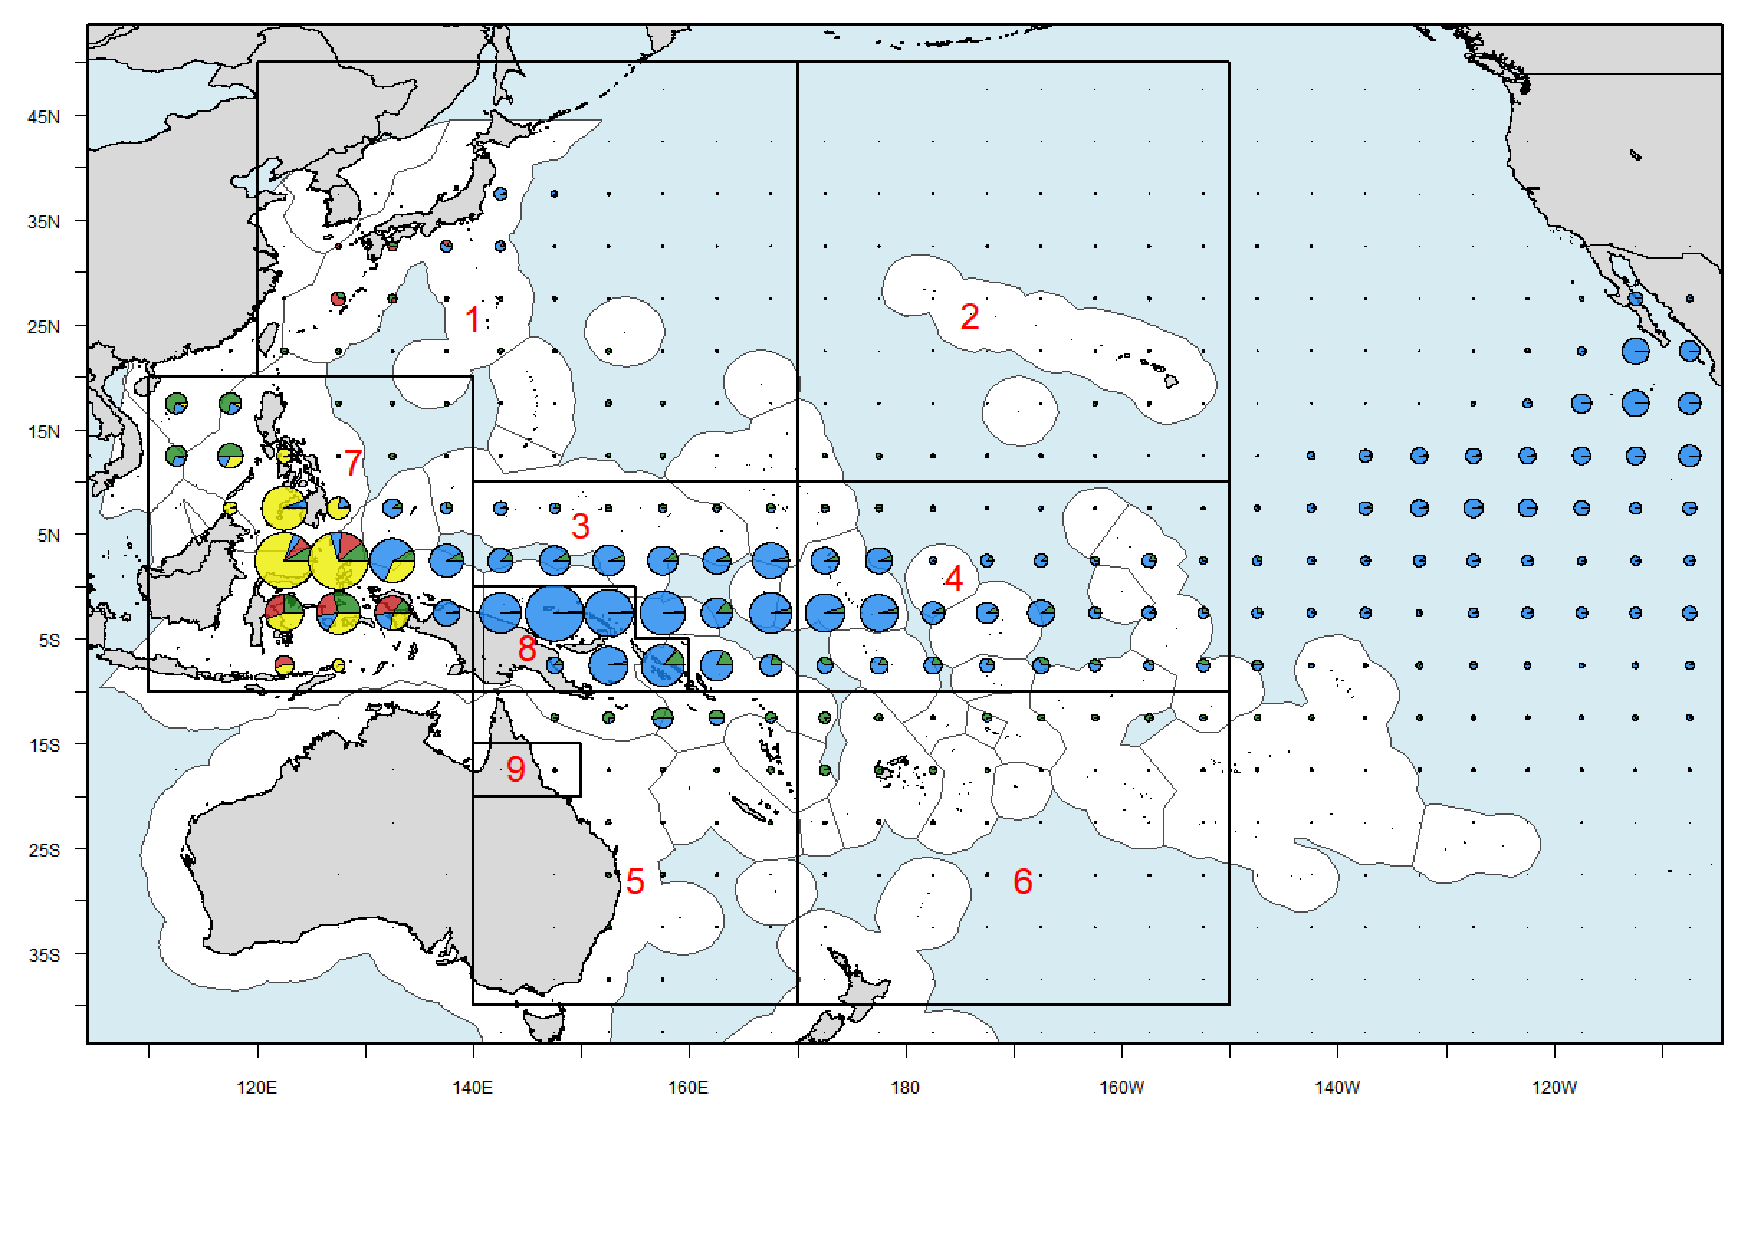
\includegraphics[height=0.82\textheight]{region_map_9}
\end{frame}

% ______________________________________________________________________________

\begin{frame}{Regional Structure}
  \vspace{1ex}
  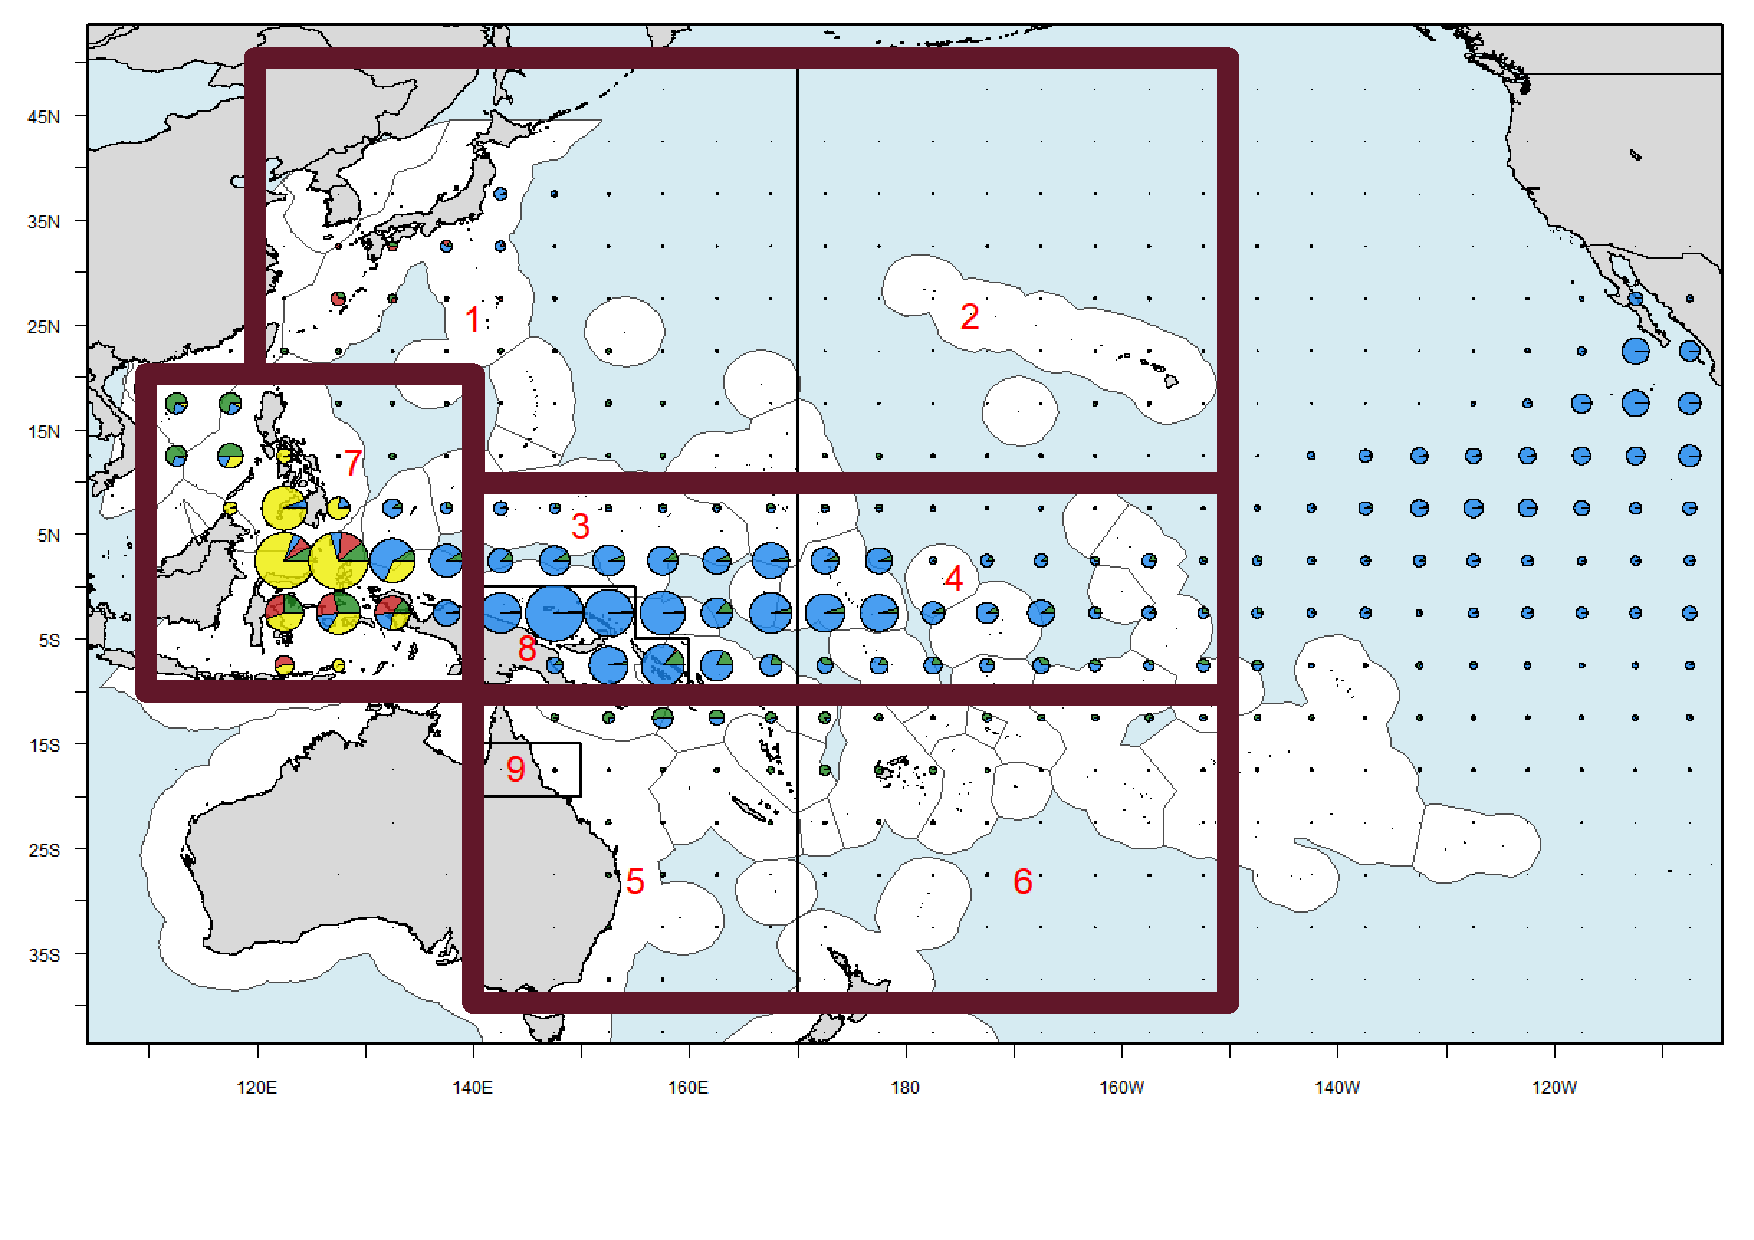
\includegraphics[height=0.82\textheight]{region_map_4}
\end{frame}

% ______________________________________________________________________________

\begin{frame}{Discussion}\small
  It would be valuable to hear your thoughts about 1 vs. 4 vs. 9 region
  model\\[4ex]

  These models
  \begin{itemize}
    \item ask different questions\\[-1ex]
    \item answer different questions\\[-1ex]
    \item will also raise different questions
  \end{itemize}
  \vspace{2ex}

  The scientific advice for the yellowfin tuna fishery is spatially explicit to
  some extent\\[4ex]

  The main assessment model could still have a coarse resolution, if augmented\\
  with advice based on high-resolution analyses to address local questions
  \vspace{4ex}
\end{frame}

\end{document}
